\chapter{Finite-part Integration}
\label{ch_3}

 \hspace{\parindent} In this chapter, we will discuss the theory of the finite-part integration \cite{galapon2017problem} and its implementation for the exact evaluation of the generalized Stieltjes transform of a function with an entire complex extension \cite{tica2018finite, tica2019finite}, and to the function with competing singularities on its complex extension \cite{doi:10.1063/5.0038274}. Before we start the discussion about the method, we will first discuss the finite-part itself. Then, we will obtain the complex contour integral representation of the finite-part integral. Finally, we will demonstrate the method of finite-part integration to evaluate the generalized Stieltjes transform expressed in equation \eqref{1.1}.


For uniformity from now on, we will use the following notations, $\mathbb{Z}$ denotes the set of integers; $\mathbb{Z}^+$, the positive integers; $\mathbb{Z}^-$, the negative integers; $\mathbb{Z}^+_0$, the positive integers including $0$; $\mathbb{Z}^-_0$, the negative integers including $0$.
 
 
\section{Finite Part of the Divergent Integrals}

Divergent integrals are not new in many areas in physics and engineering \cite{bonnet1999boundary, frankel2006generalizing, frankel2007regularization}. Usually, the divergence is due to a non-integrable singularity located inside the interval of integration. For example, the family of divergent integrals in the form of
\begin{equation} \label{FoD}
    \int_{a}^{b} \frac{f(x)}{(x-x_0)^{n+1}} \, \mathrm{d}x, \quad -\infty < a < x-0 < b < \infty, \quad n \in \mathbb{Z}_0^{+}
\end{equation}
for some function $f(x)$ that does not vanish at $x=x_0$. To assign a meaningful value for the above integral, one may remove the non-integrable point $x_0$ and modified the form of the divergent integral \eqref{FoD} into 
\begin{equation}
    \lim_{\epsilon \to 0} \left[ \int_{a}^{x_0 - \epsilon} \frac{f(x)}{(x-x_0)^{n+1}} \, \mathrm{d}x + \int_{x_0 + \epsilon}^{b} \frac{f(x)}{(x-x_0)^{n+1}} \, \mathrm{d}x \right],
\end{equation}
where a finite value is obtained and assigned as the value of the divergent integrals whenever the limit exist. Under the continuity condition on $f(x)$, the limit will only exists for the case $n=0$, which leads to the definition of the well-known Cauchy Principal Value (CPV),
\begin{equation}
    \mathrm{CPV}\int_{a}^{b} \frac{f(x)}{x-x_0} \, \mathrm{d}x = \lim_{\epsilon \to 0} \left[ \int_{a}^{x_0 - \epsilon} \frac{f(x)}{x-x_0} \, \mathrm{d}x + \int_{x_0 + \epsilon}^{b} \frac{f(x)}{x-x_0} \, \mathrm{d}x \right].
\end{equation}
For the other cases, $n=1,2, \dots$, the limits will no longer exist. However, we can still assign a meaningful value from it by performing a usual integration without considering the behavior of the integrand on the singularity. For example, when $n=1$ and $f(x)$ is some constant function $c$, we will obtain the equality
\begin{equation}
    \lim_{\epsilon \to 0} \left[ \int_{a}^{x_0-\epsilon} + \int_{x_0+\epsilon}^{b} \right] \frac{c}{(x-x_0)^{2}} \, \mathrm{d}x = - \left[ \frac{c}{b-x_0} + \frac{c}{x_0-a} \right] + \frac{2}{\epsilon}.
\end{equation}
It can be observed that the limit will not exist due to the diverging term $2/\epsilon$. To assign a finite part value on this divergent integral, we will drop the diverging terms when $\epsilon \to 0$,
\begin{equation}
    \mathrm{FPI} \int_{a}^{b} =  - \left[ \frac{c}{b-x_0} + \frac{c}{x_0-a} \right].
\end{equation}
The same way can be applied for the other value of $n$ and $f(x)$ to assign a finite value to the divergent integral. This manner of assigning finite value to the divergent integrals is due to Hadamard, and the finite value is known as the Hadamard finite-part or the Finite-Part Integral (FPI).

In \cite{galapon2016cauchy}, under a certain conditions, the divergent integral in \eqref{FoD} was assigned to a complex contour integral and refer to it as Analytic Principal Value (APC). It is mathematically express as
\begin{equation}
    \bbint{a}{b} \frac{f(x)}{(x-x_0)^{n+1}} \, \mathrm{d}x = \frac{1}{2} \left[ \mathrm{Int}^{+}(x_0) + \mathrm{Int}^{-}(x_0) \right]
\end{equation}
where APV is denoted with the symbol $\bbint{a}{b}$ and $\mathrm{Int}(x_0)$ is a complex contour integration with the form
\begin{equation}
    \mathrm{Int}^{\pm}(x_0) = \int_{C^{\pm}} \frac{f(z)}{(z-x_0)^{n+1}} \, \mathrm{d}z.
\end{equation}


\begin{figure}
    \centering
    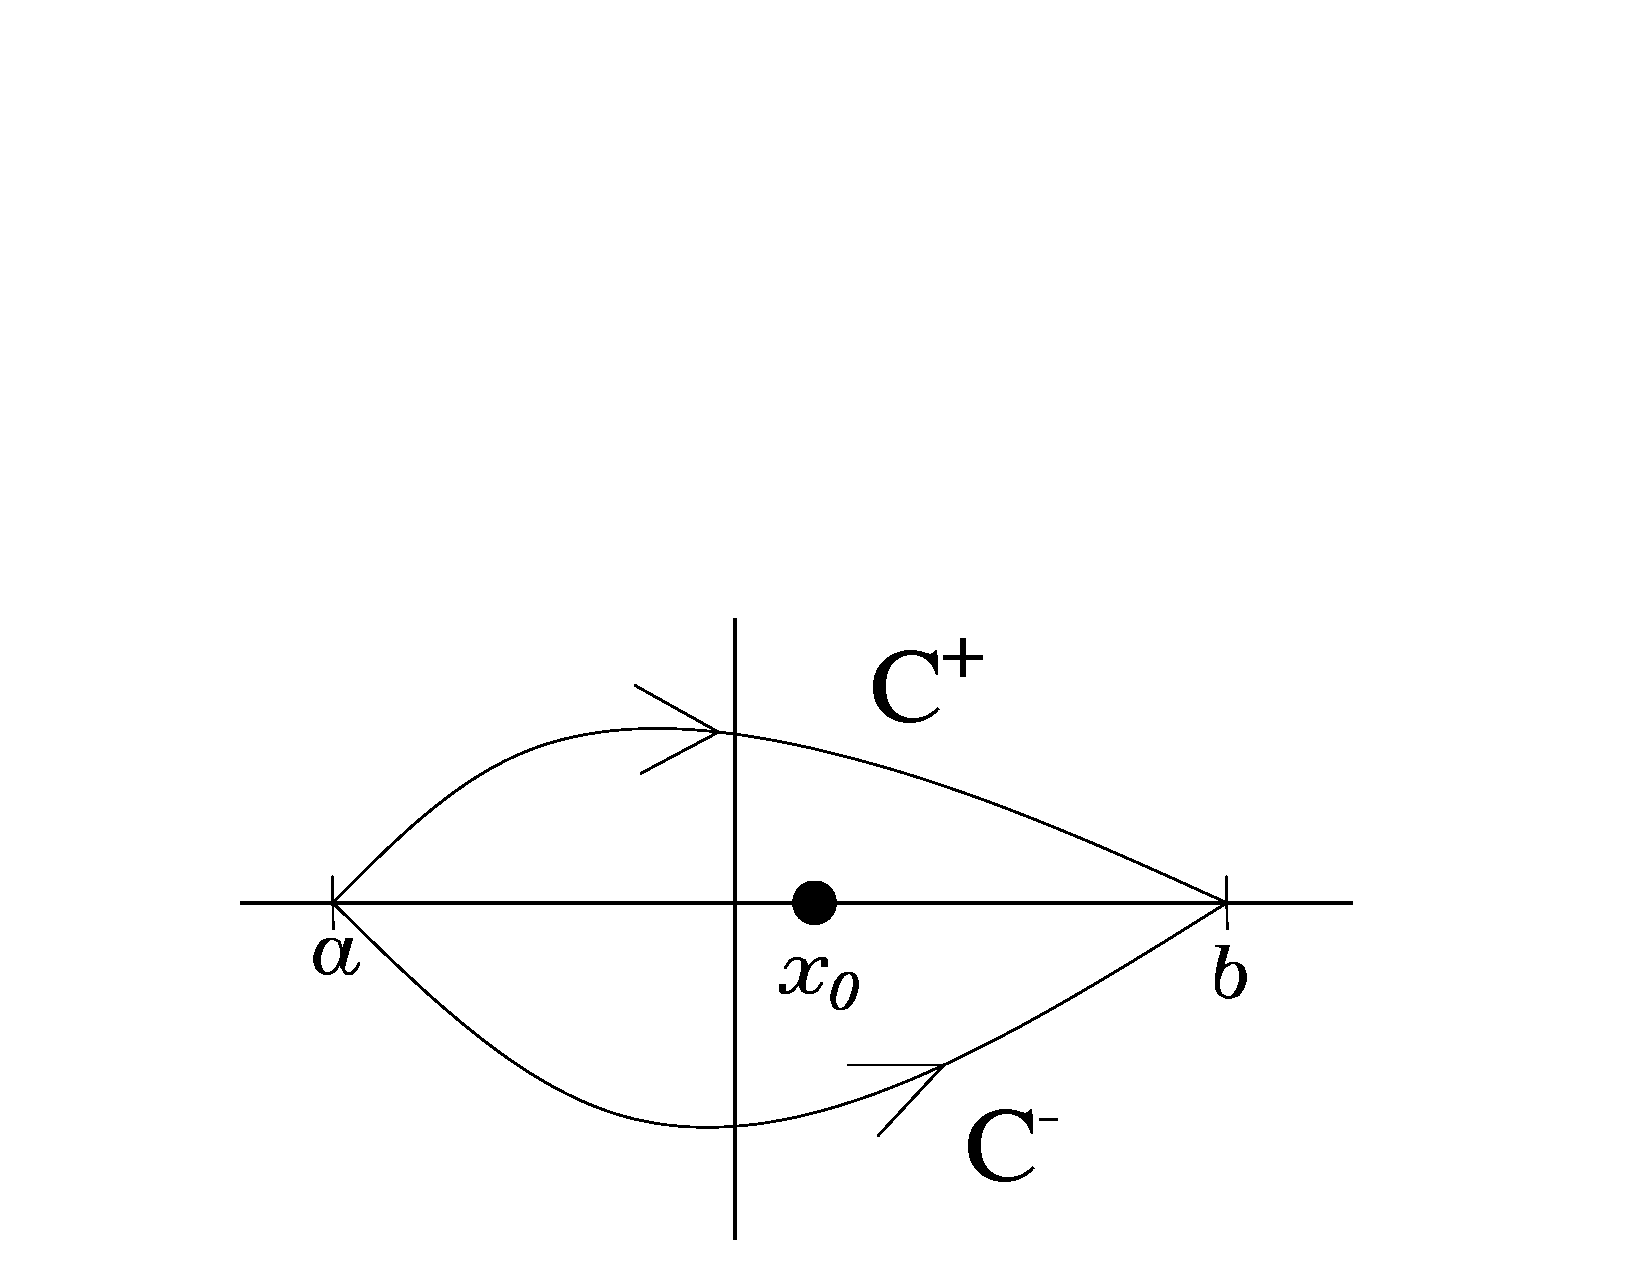
\includegraphics[width=.75\textwidth]{qwer.pdf}
    \caption{The contour $C^{+}$ is an arbitrary contour that runs from $a$ to $b$ above the singularity located at $z=x_0$. While contour $C^{-}$ is an arbitrary contour start from $a$ to $b$ below the singularity at $z=x_0$.}
    \label{APVc}
\end{figure}

\noindent The contour $C^{+}$ runs from $z=a$ to $z=b$ above the singularity $z=x_0$, while $C^{-}$ runs with the same path but below the singularity $z=x_0$, which is shown in Figure \ref{APVc}. It was shown in the same paper that the APV is an equivalent but distinct representation of the Cauchy principal value for $n=0$ and the Hadamard finite-part integral for positive integers $n$. This result gives rise to the heart of the finite-part integration, the complex contour integral representation of the finite part of the divergent integral.

\section{Evaluation of Finite-part Integral}

Consider a standard Stieltjes transform 
 \begin{equation}
     S[f] = \int_0^{\infty} \frac{f(x)}{\omega + x}\, \mathrm{d}x.
\end{equation}
Expanding the kernel $\omega + x$ for small $\omega$ at the origin 
\begin{equation}
    \frac{1}{\omega+x} = \sum_{k=0}^{\infty} (-1)^{k} \frac{\omega^{k}}{x^{k+1}},
\end{equation}
and evaluating the integral by means of term by term integration will result to a family of divergent integrals
 \begin{equation}
     \int_{0}^{\infty} \frac{f(x)}{x^{m+\nu}} \, \mathrm{d}x, \quad m \in \mathbb{N}, \quad 0 \leq \nu < 1, \quad 0 < a \leq \infty
     \label{4.33}
 \end{equation}
for non-integrable singularity at the origin. The divergence of this integral can be removed by replacing the lower limit of integration to some positive $\epsilon$ less than to the upper limit of integration $a$. This will give us the temporary finite-part of the divergent integral and will allow us to group the resulting integral into a pair of terms;
\begin{equation}
    \int_{0}^{a} \frac{f(x)}{x^{m+\nu}} \, \mathrm{d}x = C_\epsilon + D_\epsilon,
\end{equation}
where $C_\epsilon$ is the group of terms that have a finite value when we take the limit of $\epsilon \to 0$ and $D_\epsilon$ is the group of terms that will diverge in the same limit. Dropping the diverging part $D_\epsilon$ will result to the finite-part of the divergent integral. Thus, the limit of the converging terms $C_\epsilon$ is the assigned value of finite-part integral (FPI),
\begin{equation}
    \mathrm{FPI} \, \int_{0}^{a} \frac{f(x)}{x^{m+\nu}} \, \mathrm{d}x = \lim_{\epsilon \to 0} C_\epsilon.
\end{equation}
Equivalently, the finite-part integral can be also expressed in the form of
\begin{equation}
    \mathrm{FPI}  \int_{0}^{a} \frac{f(x)}{x^{m+\nu}} \, \mathrm{d}x, = \lim_{\epsilon \to 0} \, \left[ \int_{\epsilon}^{a} \frac{f(x)}{x^{m+\nu}} \, \mathrm{d}x - D_\epsilon \right].
    \label{FPI2}
\end{equation}
By definition, the limits of the two expression of finite-part integral always exists, and will have a value equal to zero under a certain circumstances. Now, when we extend the upper limit of integration to infinity, $a=\infty$, the finite-part is given by the limit
\begin{equation}
    \mathrm{FPI}  \int_{0}^{\infty} \frac{f(x)}{x^{m+\nu}} \, \mathrm{d}x = \mathrm{FPI} \lim_{a \to \infty} \int_{0}^{a} \frac{f(x)}{x^{m+\nu}} \, \mathrm{d}x.
\end{equation}
To guarantee the existence of the limit of the above equation, it is assumed that the $f(x)x^{-(m+\nu)}$ is integrable at infinity. The order of the evaluation of the limit should be followed strictly. 

To distinguish the familiar notation $\mathrm{FPI} \int_0^{a}$ to the the finite-part of the divergent integral in equation \eqref{4.33}, we will denote it as $\bbint{0}{a}$. This new notation indicate that  we are only dealing to the finite-part integral of the function $f(x)$ with holomorphic complex extensions.

Lastly, one may question the uniqueness of the definition of finite-part integral. To address the ambiguity in the definition, we will discuss it through examples. For example, the term $e^{1/\epsilon}$ appeared after an integration. This term will diverge as we take the limit of $\epsilon \to 0$. If we take $e^{1/\epsilon}$ as a whole, then we need to drop it, and the resulting finite-part is zero. However, if we choose to expand it as  $e^{1/\epsilon} = 1 + 1/\epsilon + 1/2! \epsilon^2 + \ldots$ before performing the limit, we will obtain a non-zero finite-part value. The finite-part value is equal to $1$ because negative exponents of $\epsilon$ will be disregarded since those terms will diverge as we take the limit of $\epsilon \to 0$. Let us consider another example, where we have $\ln (2 \epsilon)$ after performing some integration. Again, if we have taken $\ln (2 \epsilon)$  as a whole, it will give us a zero finite-part value since $\lim_{\epsilon \to 0} \ln(2 \epsilon) = -\infty$. Also, if we take $\ln (2\epsilon) = \ln(2) + \ln(\epsilon)$, it can give us a non-zero finite-part value equal to $\ln(2)$. The term $\ln(\epsilon)$ will be drop since it will diverge as we take the limit of $\epsilon \to 0$. Now, we ask the question, which of the two in each example is the finite-part? This ambiguity of finite-part can be resolve by requiring that the divergent part $D_{\epsilon}$ only take the form of at most the sum of inverse powers of $\epsilon$ and powers of the logarithm $\ln{\epsilon}$. This requirement will result in the finite-part value $1$ and $\ln (2)$ as the desired finite-part for the two examples, respectively. In consequence, the function $f(x)$ is required to have an expansion about $x=0$ in the calculation of finite-part. Similarly, $f(x)$ should be infinitely differentiable at the origin so that it will have a representation in some neighborhood of the origin written as $f(x) = \sum_{k=0}^{\infty} a_k x^{k}$.


\begin{figure}
    \centering
    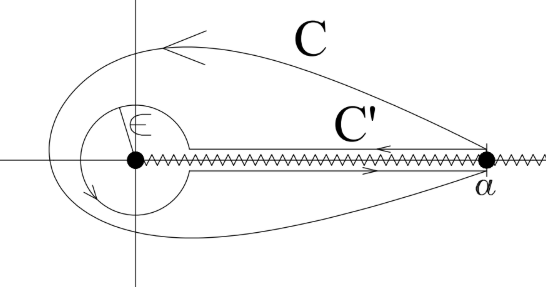
\includegraphics[width=.75\textwidth]{c30.PNG}
    \caption{The contour of integration. The contour $C$ does not enclose any poles or branch points of $f(z)$.}
    \label{ch31}
\end{figure}

\section{Complex Contour Integral Representation of the Finite-part Integral}

Now, it's time to present the heart of the finite-part integration, the contour integral representation of the finite-part integral in the complex plane \cite{galapon2017problem, galapon2016cauchy}. Lifting the finite-part integral to the complex plane requires $f(x)$ to have an analytic complex extension $f(z)$. This contour integral representation is in the form of $\int_{C} f(z) G(z) z^{-m-\nu}$, where $G(z)$ is the function that will induce a branch cut, when necessary. This branch cut runs along the path of integration. The contour $C$ will runs from $a$ and goes back to $a$ to enclose the segment [$0, a$] as shown in Figure \ref{ch31}. The figure is obtained from \cite{doi:10.1063/5.0038274}. The contour $C$ will be deformed in such a way it will straddle the branch cut. The process will lead to a complex contour integral representation of the finite-part integral. Take note that the contour $C$ should not enclosed any pole from $f(z)$ or intersect any branch cuts of $f(z)$.

From the above process, we see that the function $G(z)$ will solely depend on the value of $\nu$. When the value of $\nu$ is zero, the finite-part integral will have a pole in its complex extension. Thus, we need to induce a branch cut that runs along the positive real axis, and we choose that branch cut is from the complex logarithm $\log z$. For the case of $\nu \neq 0$, we do not need to induce a branch cut since the complex extension of the finite-part integral will have a branch point, and we need to choose that the branch cut runs along the positive real axis. Therefore, it is important to know the nature of the divergence of the integrand in the application of finite-part integration. 

The contour integral representation of the two cases and its proof is obtained from \cite{galapon2017problem}.

\subsection{Pole Singularity}

\begin{proposition}
Let $f(x)$ be (m+1) continuously differentiable in the interval $[0,a]$ and $M=sup\{ |f^{(m)}(x)|, x \in [0,a]\} < \infty$. If $f(0) \neq 0$ then we have the finite part integral
\begin{align}
\begin{split}
 \bbint{0}{a} \frac{f(x)}{x^{m+1}} \, \mathrm{d}x & = \lim_{\epsilon \to 0} \Bigg[ \int_\epsilon^a \frac{f(x)}{x^m} \, \mathrm{d}x \\& - \sum_{k=0}^{m-2} \frac{f^{(k)}(0)}{k! (m-1-k)}\frac{1}{\epsilon^{m-1-k}} + \frac{f^{(m-1)}(0)}{(m-1)!} \ln \epsilon \Bigg]
    \label{3.7}
\end{split}
\end{align}
for all $m \in \mathbb{N}$.
\end{proposition}

\begin{proof}
Consider the convergent integral 
\begin{equation}
    \int_\epsilon^a \frac{f(x)}{x^{m+1}} \, \mathrm{d}x
    \label{3.8}
\end{equation}
for $\epsilon \in (0,a)$. Assuming that the function $f(x)$ is differentiable up to $(m+1)$th order. From that assumption, we can write the function $f(x)$ in the form of 
\begin{equation}
    f(x) = \sum_{k=0}^{m} \frac{f^{(k)}(0)}{k!} x^{k} + R_{m+1}(x).
\end{equation}
Substituting the expansion to equation \eqref{3.8} will result to
\begin{equation}
    \int_\epsilon^a \frac{f(x)}{x^{m+1}} \, \mathrm{d}x = \int_\epsilon^{a} \frac{\mathrm{d}x}{x^m+1} \left( \sum_{k=0}^{m-1} \frac{f^{(k)}(0)}{k!}x^{k} + \frac{f^{(m)}(0)}{m!}x^{m} + R_{m+1}(x) \right).
\end{equation}
Then, performing term by term integration will give us
\begin{align}
\begin{split}
    \int_\epsilon^a \frac{f(x)}{x^{m+1}} \, \mathrm{d}x & =- \sum_{k=0}^{m-1} \frac{f^{(k)}(0)}{k!(m-k)} \left( \frac{1}{a^{m-k}} - \frac{1}{\epsilon^{m-k}} \right) \\& +  \frac{f^{(m)}(0)}{m!} \left( \ln a - \ln \epsilon \right) + \int_\epsilon^{a}\frac{R_{m+1}(x)}{x^{m+1}} \mathrm{d}x.
    \label{3.11}
\end{split}
\end{align}
Since the $|R_{m+1}(x)| \leq M|x|^{m+1}/(m+1)! $ for some positive constant M, the integral of the remainder is bounded by 
\begin{equation}
   \left| \int_\epsilon^{a}\frac{R_{m+1}(x)}{x^{m+1}} \mathrm{d}x \right| \leq \int_\epsilon^{a}\frac{|R_{m+1}(x)|}{x^{m+1}} \mathrm{d}x \leq \frac{M}{(m+1)!} (a- \epsilon) \leq \frac{Ma}{(m+1)!}.
\end{equation}
Therefore, the integral of the remainder term exists as we take the limit of $\epsilon \to 0$. Next, we rearrange the equation \eqref{3.11} in such a way we will put the group of the diverging terms to the left and the group of the converging terms to the right as we take the limit of $\epsilon \to 0$.
\begin{align}
\begin{split}
    \int_\epsilon^a & \frac{f(x)}{x^{m+1}} \, \mathrm{d}x  - \sum_{k=0}^{m-1} \frac{f^{(k)}(0)}{k!(m-k)} \frac{1}{\epsilon^{m-k}} + \frac{f^{(m)}(0)}{m!} \ln \epsilon \\& = -\sum_{k=0}^{m-1} \frac{f^{(k)}(0)}{k!(m-k)} \frac{1}{a^{m-k}} +  \frac{f^{(m)}(0)}{m!} \ln a + \int_\epsilon^{a}\frac{R_{m+1}(x)}{x^{m+1}} \mathrm{d}x.
\end{split}
\end{align}
Finally, we reproduce the finite-part integral in equation \eqref{3.7} by taking the limit of $\epsilon \to 0$. Dropping the diverging terms in the LHS will result to Hadamard finite-part integral.
\end{proof}


\begin{theorem} \label{T3.1}
Let the complex extension, $f(z)$, of $f(x)$ be analytic in some neighbourhood of the interval $[0, a]$. If $f(0) \neq 0$ and $m = 0,1,2,...$, then
\begin{equation}
    \bbint{0}{a} \frac{f(x)}{x^{m+1}} \, \mathrm{d}x = \frac{1}{2 \pi i} \int_{C} \frac{f(z)}{z^{m+1}} (\log z - \pi i) \, \mathrm{d}z
\end{equation}
where $\log z$ is the complex logarithm whose branch cut is the positive real axis and $C$ is the contour straddling the branch cut of $\log z$ starting from $a$ and ending at $a$ itself, as depicted in Figure \ref{ch31}.
\end{theorem}

\begin{proof}
First, we will consider the complex contour integral 
\begin{equation}
    \int_{C} \frac{f(z)}{z^{m+1}} \log z \, \mathrm{d}z
\end{equation}
where the contour $C$ is shown in the Figure \ref{ch32} and will be deformed into $C'$. The complex contour integral will be evaluated along the deformed $C'$ and will give us
\begin{equation}
    \int_{C} \frac{f(z)}{z^{m+1}} \log z \, \mathrm{d}z = \int_a^{\epsilon} \frac{f(x) \log x}{x^{m+1}} \, \mathrm{d}x + \int_{\epsilon} \frac{f(z) \log z}{z^{m+1}} \, \mathrm{d}z + \int_\epsilon^a \frac{f(x) \log (x \mathrm{e}^{2 \pi i})}{x^{m+1}} \, \mathrm{d}x.       
\end{equation}
The first term represent the path above the branch cut  induced by $\log z$, the second is the small circle about the origin, and the third term is the path below the branch cut. Using the logarithmic property, it will give as the relation $\log \,x = \log \, x + 2 \pi i$ and will simplify the equation into 
\begin{equation}
    \int_{C} \frac{f(z)}{z^{m+1}} \log z \, \mathrm{d}z = 2 \pi i \int_{\epsilon}^a \frac{f(x)}{x^{m+1}} \, \mathrm{d}x + \int_{\epsilon} \frac{f(z) \log z}{z^{m+1}} \, \mathrm{d}z  . 
    \label{3.18}
\end{equation}

Now, we will evaluate the integral along the small circle by expanding first the function $f(z)$ at $z=0$, which give us
\begin{equation}
    f(z) = \sum_{k=0}^{m} \frac{f^{(k)}(0)}{k!} z^k + \mathcal{O}(z^{m+1}), m = 0,1,....
\end{equation}
since by assumption it is analytic at $z=0$. Substituting it back to the integral and using the parameterization $z = \epsilon \mathrm{e}^{i \theta}$, $0 \leq \theta < 2 \pi$ and via logarithmic property, we use the relation $\log(x \mathrm{e}^{i \theta}) = \log x + i \theta$  and obtain
\begin{align}
\begin{split}
    \int_{\epsilon} \frac{f(z) \log z}{z^{m+1}} \,  \mathrm{d}z & = \sum_{k=0}^m \frac{f^{(k)}(0)}{k!} \frac{1}{\epsilon^{m-k}} \bigg[ i \ln \epsilon \int_0^{2 \pi} \mathrm{e}^{-i(m-k)\theta} \mathrm{d}\theta \\& - \int_0^{2 \pi} \mathrm{e}^{-i(m-k)\theta} \theta \mathrm{d}\theta  \bigg] + \mathcal{O}(\epsilon).
    \label{3.20}
\end{split}
\end{align}
the above integral will be evaluated using these known integrals:
\begin{equation}
    \int_0^{2 \pi} \mathrm{e}^{-i(m-k)\theta} \, \mathrm{d}\theta = 
    \begin{cases} 
      0, & m \neq k \\
      2 \pi, & m = k
   \end{cases}
\end{equation}
and
\begin{equation}
    \int_0^{2 \pi} \mathrm{e}^{-i(m-k)\theta} \theta \, \mathrm{d}\theta =     \begin{cases} 
      \frac{2 \pi i}{m-k}, & m \neq k \\
      2 \pi^2, & m = k
   \end{cases} .
\end{equation}
Substituting the integrals above to equation \eqref{3.20}, will result to
\begin{align}
\begin{split}
    \int_{\epsilon} \frac{f(z) \log z}{z^{m+1}} \,  \mathrm{d}z & = 2 \pi i \left[ \frac{f^{(m)}(0)}{m!} \ln \epsilon - \sum_{k=0}^{m-1} \frac{f^{(k)}(0)}{k!(m-k) \epsilon^{m-k}} \right] \\& - 2 \pi^{2} \frac{f^{(m)}(0)}{(m-1)!} + \mathcal{O}(\epsilon).
    \label{3.23}
\end{split}
\end{align}
Since we already evaluated the integral along the small circle about the origin, we will substitute it back to the contour integral in equation \eqref{3.18} that will result to
\begin{align}
\begin{split}
     \int_{C} & \frac{f(z)}{z^{m+1}} \log z \, \mathrm{d}z = 2 \pi i \bigg[ \int_{\epsilon}^a \frac{f(x)}{x^{m+1}} \, \mathrm{d}x +  \frac{f^{(m)}(0)}{m!} \ln \epsilon \\&  - \sum_{k=0}^{m-1} \frac{f^{(k)}(0)}{k!(m-k) \epsilon^{m-k}} \bigg] - 2 \pi^{2} \frac{f^{(m)}(0)}{(m)!} + \mathcal{O}(\epsilon).
    \label{3.24}
\end{split}
\end{align}
We will manipulate the last term in the right-hand side of the equation as
\begin{equation}
    2 \pi^{2} \frac{f^{(m)}(0)}{(m)!} = \frac{\pi}{i} \int_{C} \frac{f(z)}{z^{m+1}} \, \mathrm{d}z = -\pi i \int_C \frac{f(z)}{z^m} \, \mathrm{d}z.
\end{equation}
Substituting the manipulated last term to the equation \eqref{3.24} and dividing both sides by $2 \pi i$ will result to 
\begin{align}
\begin{split}
     \frac{1}{2 \pi i}\int_{C} & \frac{f(z)}{z^{m+1}} (\log z - \pi i) \, \mathrm{d}z = \int_{\epsilon}^a \frac{f(x)}{x^{m+1}} \, \mathrm{d}x +  \frac{f^{(m)}(0)}{m!} \ln \epsilon \\&  - \sum_{k=0}^{m-1} \frac{f^{(k)}(0)}{k!(m-k) \epsilon^{m-k}} + \mathcal{O}(\epsilon).
\end{split}
\end{align}
Taking the limit of $\epsilon \to 0^{+}$, we recognize that the right-hand side is the definition of the Hadamard finite part in equation \eqref{3.7}. Therefore, 
\begin{equation}
    \bbint{0}{a} \frac{f(x)}{x^{m+1}} \, \mathrm{d}x = \frac{1}{2 \pi i} \int_C \frac{f(z)}{z^{m+1}} (\log z - \pi i) \, \mathrm{d}z,
\end{equation}
for  $m = 0, 1,2, ...$.
\end{proof}

\subsection{Branch Point Singularity}
\begin{proposition}
Let $f(x)$ be n continuously differentiable in the interval $[0,a]$ and $M=sup\{ |f^{(n)}(x)|, x \in [0,a]\} < \infty$. If $f(0) \neq 0$ then we have the finite part integral
\begin{align}
\begin{split}
    \bbint{0}{a} \frac{f(x)}{x^{n+\nu}} \, \mathrm{d}x & = \lim_{\epsilon \to 0^{+}} \Bigg[ \int_\epsilon^a \frac{f(x)}{x^m} \, \mathrm{d}x \\& - \sum_{l=0}^{m-1} \frac{f^{(l)}(0)}{l! (n+\nu-l-1)}\frac{1}{\epsilon^{n+\nu-l-1}} \Bigg] 
\label{P2}
\end{split}
\end{align}
for all $n \in \mathbb{N}$ and $\nu \in (0,1)$.
\end{proposition}

\begin{proof}
Similar to the case of pole singularity, we will consider an integral in the form of 
\begin{equation}
    \int_\epsilon^a \frac{f(x)}{x^{n+ \nu}} \, \mathrm{d}x
    \label{3.29}
\end{equation}
for $\epsilon \in (0,a)$. Since we let $f(x)$ to be $n$th differentiable along the integral, we can expand it at the origin via the Taylor series expansion given by
\begin{equation}
    f(x) = \sum_{k=0}^{n-1} \frac{f^{(k)}(0)}{k!} \, x^{k} + R_{n}(x)
\end{equation}
Substituting this expansion to the integral we considered in \eqref{3.29}, and integrating it, will result to
\begin{align}
\begin{split}
    \int_\epsilon^a \frac{f(x)}{x^{n+ \nu}} \, \mathrm{d}x & = \sum_{k=0}^{n-1} \frac{f^{(k)}(0)}{k!(k-n-\nu+1)} \, \left( \frac{1}{a^{n+\nu-k-1}} - \frac{1}{\epsilon^{n+\nu-k-1}} \right) \\& + \int_\epsilon^a \frac{R_{n}(x)}{x^{n+\nu}} \, \mathrm{d}x. 
    \label{3.31}
\end{split}
\end{align}
Next, we need to find out if the remainder term has a finite limit as we take $\epsilon \to 0$. Using the bound for the remainder term $R_n{x} \leq M |x|^{n}/n!$ for some positive constant $M$.  The bound for the integral involving the remainder is given by
\begin{equation}
    \left| \int_\epsilon^a \frac{R_{n}(x)}{x^{n+\nu}} \, \mathrm{d}x \right| \leq \int_\epsilon^a \frac{|R_{n}(x)|}{x^{n+\nu}} \, \mathrm{d}x \leq \frac{M}{n!(1-\nu)} (a^{1-\nu} - \epsilon^{1-\nu})
\end{equation}
since $\nu \in (0,1)$, the integral consisting of the the remainder term exists as $\epsilon \to 0$. Now, we will rearrange the terms on equation \eqref{3.31} in such away, the group of the diverging in term is in the left-hand side and the group of converging term is in the right-hand side as we take the limit of $\epsilon \to 0$. The resulting equation is 
\begin{align}
\begin{split}
    \int_\epsilon^a & \frac{f(x)}{x^{n+ \nu}} \, \mathrm{d}x + \sum_{k=0}^{n-1} \frac{f^{(k)}(0)}{k!(k-n-\nu+1)} \, \frac{1}{\epsilon^{n+\nu-k-1}} \\&  = \sum_{k=0}^{n-1} \frac{f^{(k)}(0)}{k!(k-n-\nu+1)} \, \frac{1}{a^{n+\nu-k-1}} + \int_\epsilon^a \frac{R_{n}(x)}{x^{n+\nu}} \, \mathrm{d}x. 
\end{split}
\end{align}
 Therefore, we reproduced the equation in equation $\eqref{P2}$.
\end{proof}

\begin{theorem}\label{T3.2}
Let the complex extension, $f(z)$, of $f(x)$ be analytic in some neighbourhood of the interval $[0, a]$. If $f(0) \neq 0$ for all $n \in \mathbb{N}$ and $0 < \nu < 1$, then 
\begin{equation}
    \bbint{0}{a} \frac{f(x)}{x^{n+\nu}} \, \mathrm{d}x = \frac{1}{\mathrm{e}^{-2 \pi \nu i}-1} \int_C \frac{f(z)}{z^{n+\nu}} \, \mathrm{d}z
\end{equation}
where the branch of $z^{-\nu}$ is such that it is positive on top of the positive real axis and the contour $C$ is the contour straddling the branch cut of $z^{-\nu}$ starting from $a$ and ending at $a$ itself, as depicted in Figure \ref{ch31}.
\end{theorem}
\begin{proof}
In order to prove the theorem, we will consider the complex integral
\begin{equation}
    \int_C \frac{f(z)}{z^{n+\nu}} \, \mathrm{d}z
\end{equation}
where the contour is shown in Figure \ref{ch32}. The contour will be deformed as $C'$ and evaluating it
\begin{align}
\begin{split}
    \int_C \frac{f(z)}{z^{n+\nu}} \, \mathbb{d}z & = \int_{a}^{\epsilon} \frac{f(x)}{x^{n+\nu}} \, \mathrm{d}x + \int_{\epsilon} \frac{f(z)}{z^{n+\nu}} \, \mathrm{d}z + \int_{a}^{\epsilon} \frac{f(x)}{x^{n+\nu} \mathrm{e}^{2 \pi \nu}} \, \mathrm{d}x \\& = (\mathrm{e}^{-2 \pi \nu i}-1) \int_{a}^{\epsilon} \frac{f(x)}{x^{n+\nu}} \, \mathrm{d}x + \int_{\epsilon} \frac{f(z)}{z^{n+\nu}} \, \mathrm{d}z.
    \label{3.36}
\end{split}
\end{align}
For the evaluation of the integral along the circle about the origin, we will have a parameterization of $z = \epsilon \mathrm{e}^{i \epsilon}$, $0 \leq \theta \leq 2 \pi$. Moreover, since we assume that $f(z)$ is analytic along the contour. We can expand $f(z)$ it as a Taylor series at the origin, given by
\begin{equation}
    f(z) = \sum_{k=0}^{n-1} \frac{f^{(k)}(0)}{k!}(\epsilon \mathrm{e}^{i \theta})^{k} + \mathcal{O}((\epsilon \mathrm{e}^{i \theta})^{n}).
\end{equation}
From that, the integral along the circle about the origin is evaluated to be
\begin{align}
\begin{split}
	\int_{\epsilon} & \frac{f(z)}{z^{n+\nu}}\mathrm{d}z = \int_{0}^{2\pi}\frac{1}{\left(\epsilon e^{i\theta}\right)^{n+\nu}}\left(\sum_{k=0}^{n-1}\frac{f^{k}(0)}{k!}\left(\epsilon e^{i\theta}\right)^{k}+\mathcal{O}\left(\left(\epsilon e^{i\theta}\right)^{n}\right)\right)\epsilon i e^{i\theta}\mathrm{d}\theta
	\\& =  \sum_{k=0}^{n-1}\frac{f^{(k)}(0)}{k!\,\epsilon^{n+\nu-k-1}}\,i\int_{0}^{2\pi} e^{-i\theta(n+\nu-k-1)}\mathrm{d}\theta + i\,\epsilon^{1-\nu} \int_{0}^{2\pi}\mathcal{O}\left(\left( e^{i\theta}\right)^{1-\nu}\right)\mathrm{d}\theta.
\end{split}
\end{align}
Performing the integration
\begin{equation}
	\int_{\epsilon}\frac{f(z)}{z^{n+\nu}}\mathrm{d}z = -\sum_{k=0}^{n-1}\frac{f^{(k)}(0)}{k!\,\left(n+\nu-k-1\right)\,\epsilon^{n+\nu-k-1}}\left(e^{-2\pi\nu i}-1\right) + \mathcal{O}(\epsilon^{1-\nu}).
	\label{3.39}
\end{equation}
Since we already simplify the integral along the circle, we will substitute it back to equation $\eqref{3.36}$. Taking the limit as $\epsilon \to 0^{+}$ will make the order term vanishes since $\nu < 1$. Then, dividing both sides by $\mathrm{e}^{-2 \pi \nu i} -1$ will result to
	\begin{equation}
		\frac{1}{\left(e^{-2\pi\nu i}-1\right)}\int_{C}\frac{f(z)}{z^{n+\nu}}\mathrm{d}z =\lim_{\epsilon\to 0}\left( \int_{\epsilon}^{a}\frac{f(x)}{x^{n+\nu}}\mathrm{d}x -\sum_{k=0}^{n-1}\frac{f^{(k)}(0)}{k!\,\left(n+\nu-k-1\right)\,\epsilon^{n+\nu-k-1}}\right).
	\end{equation}
The RHS of the above equation is recognized to be the Hadamard finite-part integration according to \eqref{P2}. Thus, we obtain the contour integral representation of the finite-part integral for the branch point singularity. 
\end{proof}


\section{Finite-part  Integration  of  the  Generalized  Stieltjes  Transform  of an Entire  Function}

In this section, we will show how we implement the method to exactly evaluate the generalized Stieltjes transform of an entire function with an integral \cite{tica2018finite} and non-integral orders \cite{tica2019finite}.

\subsection{Finite-Part Integration of the Generalized Stieltjes Transform of an Entire Function with Integral Order}


%Figure
\begin{figure}
    \centering
    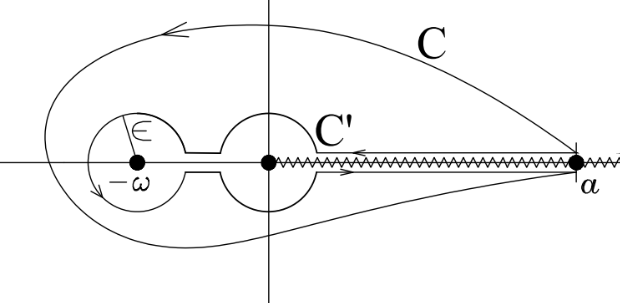
\includegraphics[width=.75\textwidth]{c31.PNG}
    \caption{The contour of integration with pole at $-\omega$, branch point at the origin, and branch cut runs from $(0,\infty)$. The contour encloses the pole at $-\omega$.}
    \label{ch32}
\end{figure}

Consider an incomplete generalized Stieltjes transform of integral order 
\begin{equation}\label{lb}
	S_{n}^{a}[f(x)] = \int_{0}^{a}\frac{f(x)}{(\omega+x)^{n}}\mathrm{d}x,
\end{equation} 
where $f(x)$ has an entire complex extension. We will have a pole at $z = -\omega$, when the integral is lifted to the complex plane. Recall from the previous discussion, we need to induce a branch cut along the positive real axis. From that, we will consider a contour integral 
\begin{equation}
    \int_C \frac{f(z)}{(\omega +z)^{n}} \log z \, \mathrm{d}z
\end{equation}
where the contour $C$ if in the Figure \ref{ch32}. Deforming the contour $C$ to $C'$ and evaluating it, will give us the equation
\begin{align}
\begin{split}
    \int_C & \frac{f(z)}{(\omega +z)^{n}} \log z \, \mathrm{d}z = \int_{a}^{\epsilon} \frac{f(x)}{(\omega +x)^{n}} \log x \mathrm{d}x + \int_\epsilon  \frac{f(z)}{(\omega +z)^{n}} \log z \, \mathrm{d}z \\& + \int_{\epsilon}^{a} \frac{f(x)}{(\omega +x)^{n}} (\log x + 2 \pi i) \mathrm{d}x + 2 \pi i \, \mathrm{Res} \left[\frac{f(z)}{(\omega +z)^{n}} \log z \,  \right]_{z=-\omega}.
\end{split}
\end{align}
Letting $\epsilon \to 0$ will make the term with the integral along the circle vanish that can be shown using L'hopitals rule. Now, combining similar terms will further simplify the equation
\begin{align}
\begin{split}
    \int_C & \frac{f(z)}{(\omega +z)^{n}} \log z \, \mathrm{d}z = 2 \pi i \int_{\epsilon}^{a} \frac{f(x)}{(\omega +x)^{n}} \mathrm{d}x  \\& + 2 \pi i\mathrm{Res} \left[\frac{f(z)}{(\omega +z)^{n}} \log z \,  \right]_{z=-\omega}.
\end{split}
\end{align}
Rearranging the equation in such a way we obtain the generalized Stieltjes transform in equation \eqref{lb} and dividing both sides by $2 \pi i$ will result to
\begin{align}
\begin{split} \label{3.47}
    \int_{\epsilon}^{a} & \frac{f(x)}{(\omega +x)^{n}} \mathrm{d}x = \frac{1}{2 \pi i} \int_C \frac{f(z)}{(\omega +z)^{n}} \log z \, \mathrm{d}z  \\& - \mathrm{Res} \left[\frac{f(z)}{(\omega +z)^{n}} \log z \,  \right]_{z=-\omega}.
\end{split}
\end{align}
The residue can be rewritten to its differential form express by the equation
\begin{equation}
	\mathrm{Res}\left[\frac{f\left(z\right)\log z}{\left(\omega+z\right)^n}\right]_{z=-\omega}= \left. \frac{1}{\left(n-1\right)!}\frac{\mathrm{d}^{n-1}}{\mathrm{d}z^{n-1}}\left(f\left(z\right)\log z\right)\right|_{z=-\omega}.
\end{equation}
This differential form can be calculated using the Leibniz rule or the generalized product rule. Applying it will result to
\begin{align}
\begin{split}
		\mathrm{Res}&\left[\frac{f\left(z\right)\log z}{\left(\omega+z\right)^n}\right]_{z=-\omega}  = \frac{1}{\left(n-1\right)!}\sum_{k=0}^{n-1}{n-1\choose k}f^{\left(k\right)}\left(-\omega\right)\left. \frac{\mathrm{d}^{n-1-k}}{\mathrm{d}z^{n-1-k}}\log z\right|_{z=-\omega}.
\end{split}
\end{align}
Now, we will separate the $k=n-1$ term from the summation and perform the differentiation,
\begin{align}
\begin{split}
		\mathrm{Res}&\left[\frac{f\left(z\right)\log z}{\left(\omega+z\right)^n}\right]_{z=-\omega}  = \\& \quad \frac{1}{\left(n-1\right)!}\sum_{k=0}^{n-2}{n-1\choose k}f^{\left(k\right)}\left(-\omega\right)\left[\frac{\mathrm{d}^{n-2-k}}{\mathrm{d}z^{n-2-k}}\,z^{-1} \right]_{z=-\omega} \\&
		 +\, \frac{f^{\left(n-1\right)}\left(-\omega\right)}{\left(n-1\right)!}\ln \omega\, +\, \pi i\,\frac{f^{\left(n-1\right)}\left(-\omega\right)}{\left(n-1\right)!}.
\end{split}
\end{align}
Using this following relation
\begin{equation}
	\frac{\mathrm{d}^{n}\,z^{-1}}{\mathrm{d}z^{n}}=\left(-1\right)^{n}\left(n!\right)z^{-n-1}\qquad\text{and}\qquad{n-1\choose k}=\frac{\left(n-1\right)!}{k!\,\left(n-1-k\right)!},
\end{equation}
and the Cauchy integral formula,
\begin{equation}
	f^{\left(n-1\right)}\left(-\omega\right)=\frac{\left(n-1\right)!}{2\pi i}\int_{C}\frac{f\left(z\right)}{\left(\omega+z\right)^n}\mathrm{d}z
\end{equation}
we successfully evaluate the residue at $z = -\omega$
\begin{align}
\begin{split}\label{esd}
	\mathrm{Res}&\left[\frac{f\left(z\right)\log z}{\left(\omega+z\right)^n}\right]_{z=-\omega}  = -\sum_{k=0}^{n-2}\frac{f^{\left(k\right)}\left(-\omega\right)\left(n-2-k\right)!\left(\omega\right)^{k-n+1}}{k!\,\left(n-1-k\right)!} \\& \hspace{25mm}
	 +\,\,\frac{f^{\left(n-1\right)}\left(-\omega\right)}{\left(n-1\right)!}\ln\omega\;+\;\frac{\pi i}{2\pi i}\int_{C}\frac{f\left(z\right)}{\left(\omega+z\right)^n}\mathrm{d}z.
\end{split}
\end{align}
Substituting the evaluated residue \eqref{esd} into equation \eqref{3.47} will result to
\begin{align}
\begin{split} \label{piyo}
	\int_{0}^{a} & \frac{f\left(x\right)}{\left(\omega+x\right)^n}\mathrm{d}x
	=\frac{1}{2\pi i}\int_{C}\frac{f\left(z\right)\left(\log z-\pi i\right)}{\left(\omega+z\right)^n}\mathrm{d}z \\& -\frac{f^{\left(n-1\right)}\left(-\omega\right)}{\left(n-1\right)!}\ln\omega
	+\omega^{1-n}\sum_{k=0}^{n-2}\frac{f^{\left(k\right)}\left(-\omega\right)\left(\omega\right)^{k}}{k!\,\left(n-1-k\right)}.
\end{split}
\end{align}
 Thus, we show that the contribution of the residue is just 
 \begin{eqnarray} \label{Res}
 \Delta_{\mathrm{sc}}^{(n)}(\omega)&=&-\;\frac{1}{\left(n-1\right)!}f^{(n-1)}\!\left(-\omega\right)\, \ln\omega \nonumber \\
 && + \sum_{k=0}^{n-2}\frac{f^{\left(k\right)}\left(-\omega\right)}{k!\,\left(n-1-k\right) \; \omega^{n-k-1}}, \;\;\; n=2, 3, \dots.
 \end{eqnarray}
For the contour integral in the first term in the right-hand side. We will expand the binomial $\omega + z$ using the binomial expansion
\begin{equation}
	\frac{1}{\left(\omega+z\right)^{n}}=\frac{1}{z^n}\sum_{k=0}^{\infty}{{-n}\choose k}\left(\frac{\omega}{z}\right)^{k}.
\end{equation}
Inserting this expansion to equation \eqref{piyo} will result to
\begin{align}
\begin{split}
	\int_{0}^{a} & \frac{f\left(x\right)}{\left(\omega+x\right)^n}\mathrm{d}x = \frac{1}{2\pi i}\int_{C}\frac{f\left(z\right)\left(\log z-\pi i\right)}{\left(z\right)^n}\sum_{k=0}^{\infty}{{-n}\choose k}\left(\frac{\omega}{z}\right)^{k}\mathrm{d}z
	\\& \hspace{25mm}-\frac{f^{\left(n-1\right)}\left(-\omega\right)}{\left(n-1\right)!}\ln\omega
	+\omega^{1-n}\sum_{k=0}^{n-2}\frac{f^{\left(k\right)}\left(-\omega\right)\left(\omega\right)^{k}}{k!\,\left(n-1-k\right)}.
\end{split}
\end{align}
The expansion is uniformly convergent for $|z| > \omega$. Since the contour integral is uniformly convergent in that case, the interchanging of order of the integration and summation is allowed
\begin{align}
\begin{split}
	\frac{1}{2\pi i}\int_{C} & \frac{f\left(z\right)\left(\log z-\pi i\right)}{\left(\omega+z\right)^n} \mathrm{d}z
	 =\\& \sum_{k=0}^{\infty}{-n\choose k}\omega^{k}\frac{1}{2\pi i}\int_{C}\frac{f\left(z\right)\left(\log z-\pi i\right)}{z^{n+k}}\mathrm{d}z.
\end{split}
\end{align}
By the virtue of the Theorem \ref{T3.1}, we express the complex contour integral as a finite-part integral
\begin{equation}
	\sum_{k=0}^{\infty}{-n\choose k}\omega^{k}\frac{1}{2\pi i}\int_{C}\frac{f\left(z\right)\left(\log z-\pi i\right)}{z^{n+k}}\mathrm{d}z = \sum_{k=0}^{\infty}{-n\choose k}\omega^{k}\,\bbint{0}{a}\frac{f\left(x\right)}{x^{n+k}}\mathrm{d}x.
\end{equation} 
Combining all the results will lead us to the theorem found in \cite{tica2018finite}.
\begin{theorem} \label{T3.3}
 	Let the complex extension, $f(z)$, of $f(x)$ be entire. Then for all $n = 1, 2, 3, \dots$ and $0<\omega<a$, the following equality holds
 	\begin{equation}
 	\int_0^a \frac{f(x)}{(\omega + x)^n} \mathrm{d}x = \sum_{k=0}^{\infty} \binom{-n}{k} \omega^{ k} \bbint{0}{a} \frac{f(x)}{x^{k + n}}\mathrm{d}x + \Delta_{\mathrm{sc}}^{(n)}(\omega)
 	\end{equation}
 	where
 	\begin{eqnarray}\label{singular_terrmm}
 	\Delta_{\mathrm{sc}}^{(n)}(\omega)&=&-\;\frac{1}{\left(n-1\right)!}f^{(n-1)}\!\left(-\omega\right)\, \ln\omega \nonumber \\
 	&& + \sum_{k=0}^{n-2}\frac{f^{\left(k\right)}\left(-\omega\right)}{k!\,\left(n-1-k\right) \; \omega^{n-k-1}}, \;\;\; n=2, 3, \dots \label{main1sub}.
 	\end{eqnarray}
 \end{theorem}

In addition, to just explicitly show that the interchanging of order of the summation and integration is valid, we need to establish the absolute convergence of the series. To do this, we will deform the contour $C$ into a circle of radius $a$ about the origin and obtain this following bound,
 \begin{eqnarray}
 \left|\bbint{0}{a} \frac{f(x)}{x^{k+n}}\mathrm{d}x\right| &=& \left|\frac{1}{2\pi i}\int_{\mathrm{C}} \frac{f(z)}{z^{k+n}} (\log z - i\pi) \mathrm{d}z\right|\nonumber \\
 &=& \left|\frac{1}{2\pi i} \int_0^{2\pi} \frac{f(a e^{i\theta})}{a^{k + n} e^{i(k+n)\theta}} (\ln a + (\theta - \pi)i) i a e^{i\theta} \mathrm{d}\theta\right|\nonumber \\
 &\leq & \frac{1}{a^{k+n - 1}} \frac{1}{2\pi} \int_0^{2\pi} \left|f(ae^{i\theta})(\ln a + (\theta - \pi)i)  \mathrm{d}\theta\right| \nonumber \\
 &\leq& \frac{1}{a^{k+n-1}} M(a)
 \end{eqnarray}
 where $M(a) > 0$ is a finite constant independent of $k$. Finally,  We will have a bound
\begin{eqnarray}\label{delta2}
\left|\sum_{k=0}^{\infty} \binom{-n}{k} \omega^{ k} \bbint{0}{a} \frac{f(x)}{x^{k  +1}}\mathrm{d}x\right|&\leq& \sum_{k=0}^{\infty} \left|\binom{-n}{k}\right| \omega^{k} \left|\bbint{0}{a} \frac{f(x)}{x^{k  +1}}\mathrm{d}x\right| \nonumber \\
&\leq& \frac{M(a)}{a^{n-1}}\sum_{k=0}^{\infty} \binom{n+k-1}{k} \frac{\omega^{ k}}{a^{k}} \nonumber \\
&=& \frac{a M(a)}{(a - \omega)^n},
\end{eqnarray}
 for the case $a>\omega$ since the infinite series converges absolutely.

 
\subsection{Finite-Part Integration of the Generalized Stieltjes Transform of an entire function with Branch Point at the Origin}

Next, we will try to implement the method of finite-part integration to the generalized Stieltjes transform of $x^{-\nu} f(x)$  
\begin{equation}\label{bl}
		S_{n}^{a}[x^{-\nu}f(x)] = \int_{0}^{a}\frac{x^{-\nu}\,f(x)}{(\omega+x)^{n}}\mathrm{d}x,
\end{equation}
where $f(x)$ has an entire complex extension $f(z)$. Lifting the integral of interest to the complex plane will induce a branch point at the origin due to the factor $x^{-\nu}$. We choose that the branch cut runs along the positive real axis. Therefore, we will have a contour integral written as
\begin{equation}
    \int_C \frac{z^{-\nu} f(z)}{(\omega + z)^{n}} \, \mathrm{d}z
\end{equation}
where contour $C$ is shown in Figure \ref{ch32}. Similar to the previous subsection, the contour will be deformed into $C'$ and evaluated to be
\begin{align}
\begin{split}
    \int_{C} & \frac{z^{-\nu}\,f\left(z\right)}{\left(\omega+z\right)^{n}}\,\mathrm{d}z =  \int_{a}^{\epsilon}\,\frac{x^{-\nu}\,f\left(x\right)}{\left(\omega+z\right)^{n}}\,\mathrm{d}x + \int_\epsilon \frac{z^{-\nu}\,f\left(z\right)}{\left(\omega+z\right)^{n}}\,\mathrm{d}z + \\& e^{-2\,\pi \nu i} \int_{\epsilon}^a\,\frac{x^{-\nu}\,f\left(x\right)}{\left(\omega+z\right)^{n}}\,\mathrm{d}x + 2 \pi i \, \mathrm{Res}\left[\frac{z^{-\nu}\,f\left(z\right)}{\left(\omega+z\right)^{n}}\,\right]_{z=-\omega}.
\end{split}
\end{align}
Combining similar terms and letting $\epsilon \to 0$ will simplify the equation to
\begin{align}
\begin{split}
    \int_{C} & \frac{z^{-\nu}\,f\left(z\right)}{\left(\omega+z\right)^{n}}\,\mathrm{d}z = (e^{-2\,\pi \nu i} - 1) \int_{\epsilon}^{a}\,\frac{x^{-\nu}\,f\left(x\right)}{\left(\omega+z\right)^{n}}\,\mathrm{d}x \\& + 2 \pi i \, \mathrm{Res}\left[\frac{z^{-\nu}\,f\left(z\right)}{\left(\omega+z\right)^{n}}\,\right]_{z=-\omega} .
\end{split}
\end{align}
Rearranging the terms in such a way we will obtain the desired integral and dividing both sides by $e^{-2\,\pi \nu i} - 1$ will lead to
\begin{align}
\begin{split} \label{3.69}
	\int_{0}^{a}\,&\frac{x^{-\nu}\,f\left(x\right)}{\left(\omega+z\right)^{n}}\,\mathrm{d}x=\frac{1}{e^{-2\pi\,\nu\,i}-1}\int_{C}\frac{z^{-\nu}\,f\left(z\right)}{\left(\omega+z\right)^{n}}\,\mathrm{d}z\\&-\frac{2\pi\,i}{e^{-2\,\pi\,i}-1}\mathrm{Res}\left[\frac{z^{-\nu}\,f\left(z\right)}{\left(\omega+z\right)^{n}}\,\right]_{z=-\omega}.
\end{split}
\end{align}
Simplifying the factor of the second term or the residue using the Euler Identity will give us 
\begin{align}
\begin{split}
	\frac{2\pi\,i}{e^{-2\pi\,\nu\,i}-1} &=\frac{2\pi\,i}{\left(e^{-\pi\,\nu\,i}-e^{\pi\,\nu\,i}\right)\,e^{-\pi\,\nu\,i}} \\& =\frac{2\pi\,i}{-2\,i\sin\left(\pi\,\nu\right)\,e^{-\pi\,\nu\,i}} \\& =\frac{-\pi}{\sin\left(\pi\,\nu\right)\,e^{-\pi\,\nu\,i}}.
\end{split}
\end{align}
We will now evaluate the residue via the Leibniz rule
\begin{eqnarray}\nonumber
	\mathrm{Res}\left[\frac{z^{-\nu}\,f\left(z\right)}{\left(\omega+z\right)^{n}}\,\right]_{z=-\omega} &=&\frac{1}{\left(n-1\right)!}\,\frac{\mathrm{d}^{n-1}}{\mathrm{d}z^{n-1}}\,\left(\frac{f\left(z\right)}{z^{\nu}}\right)_{z=-\omega}\nonumber\\\nonumber
	&=&\frac{1}{\left(n-1\right)!}\,\sum_{k=0}^{n-1}\,{{n-1}\choose{k}}\,f^{(n-1-k)}\left(-\omega\right)\,\left.\frac{\mathrm{d}^{k}}{\mathrm{d}z^{k}}\,z^{-\nu}\,\right|_{z=-\omega},
\end{eqnarray}
and using this relation
\begin{equation}
	\frac{\mathrm{d}^{k}}{\mathrm{d}z^{k}}\,z^{-\nu}=\left(-1\right)^{k}\,\nu\left(\nu+1\right)\cdots\left(\nu+k-1\right)\,z^{-\left(\nu+k\right)}
	=\frac{\left(-1\right)^{k}\,\left(\nu\right)_{k}}{z^{\nu+k}},
\end{equation}
will further simplify the residue to
\begin{equation}
\mathrm{Res}\left[\frac{z^{-\nu}\,f\left(z\right)}{\left(\omega+z\right)^{n}}\,\right]_{z=-\omega}  = \sum_{k=0}^{n-1}\,\frac{f^{(n-1-k)}\left(-\omega\right)}{k!\,\left(n-1-k\right)!}\,\frac{\left(\nu\right)_{k}}{\omega^{\nu+k}\,e^{\pi\,\nu\,i}}.
\end{equation}
Finally, the residue is calculated and simplified to be
\begin{equation}\label{rey}
	\frac{2\pi\,i}{e^{-2\,\pi\,i}-1}\mathrm{Res}\left[\frac{z^{-\nu}\,f\left(z\right)}{\left(\omega+z\right)^{n}}\right]_{z=-\omega}=\frac{-\pi}{\sin\left(\pi\,\nu\right)\,\omega^{\nu}}\,\sum_{k=0}^{n-1}\,\frac{f^{(n-1-k)}\,\left(-\omega\right)}{k!\,\left(n-1-k\right)!}\frac{\left(\nu\right)_{k}}{\omega^{k}}
\end{equation} 
Thus, proving the $\Delta_{\mathrm{sc}}^{(n)}$ in equation \eqref{delta2}.

For the contour integral of the equation \eqref{3.69}, we will expand the binomial $(\omega + z)^{-n}$ at the origin using the binomial expansion is given by
\begin{equation}
		\frac{1}{\left(\omega+z\right)^{n}}=\frac{1}{z^n}\sum_{k=0}^{\infty}{{-n}\choose k}\left(\frac{\omega}{z}\right)^{k},
\end{equation}
where the expansion is uniformly convergent for $|z| > \omega$. Since the contour runs and uniformly convergent for $|z| > \omega$, the interchanging of order of the summation and integration is valid. Substituting and interchanging the order of summation and integration will result to 
\begin{eqnarray}\nonumber\label{riy}
	\frac{1}{e^{-2\pi\,\nu\,i}-1}\int_{C}\frac{z^{-\nu}\,f\left(z\right)}{\left(\omega+z\right)^{n}}\,\mathrm{d}z&=&\frac{1}{e^{-2\pi\,\nu\,i}-1}\int_{C}\frac{f\left(z\right)}{z^{\nu+n}}\,\sum_{k=0}^{\infty}\,{{-n}\choose{k}}\left(\frac{\omega}{z}\right)^{k}\,\mathrm{d}z\\\nonumber
	&=&\sum_{k=0}^{\infty}\,{{-n}\choose{k}}\,\frac{\omega^{k}}{e^{-2\pi\,\nu\,i}-1}\,\int_{C}\,\frac{f\left(z\right)}{z^{n+k+\nu}}\mathrm{d}z\\
	&=&\sum_{k=0}^{\infty}\,{{-n}\choose{k}}\,\omega^{k}\,\bbint{0}{a}\,\frac{f\left(x\right)}{x^{n+k+\nu}}\,\mathrm{d}x
\end{eqnarray}
where the Theorem \ref{T3.1} is used to identify the contour integral as the finite-part integral. Again, combining all the results from equation \eqref{3.69}, \eqref{rey}, and \eqref{riy} will reproduce the theorem from  \cite{tica2018finite}.

\begin{theorem}\label{T3.4}
	Let the complex extension, $f\left(z\right)$, of $f\left(x\right)$ be entire. Then for all $n=1,2,3,\dots$, $0<\omega<a$, and $0<\nu<1$, the following equality holds
	\begin{equation} \label{3.64}
	\int_{0}^{a}\,\frac{x^{-\nu}f\left(x\right)}{\left(\omega+x\right)^{n}}\,\mathrm{d}x=\sum_{k=0}^{\infty}\,{{-n}\choose{k}}\,\omega^{k}\,\bbint{0}{a}\,\frac{f\left(x\right)}{x^{n+k+\nu}}\,\mathrm{d}x+\Delta_{\mathrm{sc}}^{(n)}\left(\omega\right)
	\end{equation}
	where
	\begin{equation} \label{3.65}
	\Delta_{\mathrm{sc}}^{(n)}\left(\omega\right)=\frac{\pi}{\sin\left(\pi\,\nu\right)\,\omega^{\nu}}\,\sum_{k=0}^{n-1}\,\frac{f^{(n-1-k)}\left(-\omega\right)}{k!\,\left(n-1-k\right)!}\,\frac{\left(\nu\right)_{k}}{\omega^{k}} .
	\end{equation}
\end{theorem}

Additionally, to formally show that the interchanging of the operators is valid, it is needed to show that the series in equation \eqref{riy} of finite part integrals converges absolutely. To show that we deform the contour $C$ into a circle of radius $a$ about the origin. Thus resulting to the following bound for the finite-part integral 
\begin{eqnarray}\nonumber
\left|\bbint{0}{a} \frac{f(x)}{x^{n+k+\nu}}\mathrm{d}x\right| &=& \left|\frac{1}{e^{-2\pi\nu i}-1}\int_{\mathrm{C}} \frac{f(z)}{z^{n+k+\nu}} \mathrm{d}z\right|\nonumber \\
&=& \left|\frac{1}{e^{-2\pi\nu i}-1} \int_0^{2\pi} \frac{f(a e^{i\theta})}{a^{n + k + \nu} e^{i(n + k+\nu)\theta}} i a e^{i\theta} \mathrm{d}\theta\right|\nonumber \\
&\leq & \frac{1}{a^{n+k+\nu-1}}\left| \frac{1}{e^{-2\pi\nu i}-1}\right| \int_0^{2\pi} \left|\frac{f(ae^{i\theta})}{e^{i\nu\theta}}\right| \mathrm{d}\theta \nonumber \\
&\leq& \frac{M(a)}{a^{n+k+\nu-1}}
\end{eqnarray}
where $M(a)$ is a finite positive constant independent of $k$.  Then we have the bound
\begin{eqnarray}
\left|\sum_{k=0}^{\infty} \binom{-n}{k} \omega^{k} \bbint{0}{a} \frac{f(x)}{x^{n+k+\nu}}\mathrm{d}x\right|&\leq& \sum_{k=0}^{\infty} \left|\binom{-n}{k}\right| \omega^{k} \left|\bbint{0}{a} \frac{f(x)}{x^{k  +\nu+1}}\mathrm{d}x\right| \nonumber \\
&\leq& \frac{M(a)}{a^{\nu-1}}\sum_{k=0}^{\infty} \binom{n+k-1}{k} \frac{\omega^{ k}}{a^{n+k}} \nonumber \\
&=& \frac{
	M(a)}{a^{\nu-1}(a - \omega)^{n}},
\end{eqnarray}
provided $a>\omega$. obviously, the infinite series converges absolutely.  Therefore, the interchanging of the operators is valid.




\subsection{Finite-Part Integration of the Generalized Stieltjes Transform of
Non-integral Order of Entire Functions}

\begin{figure}
    \centering
    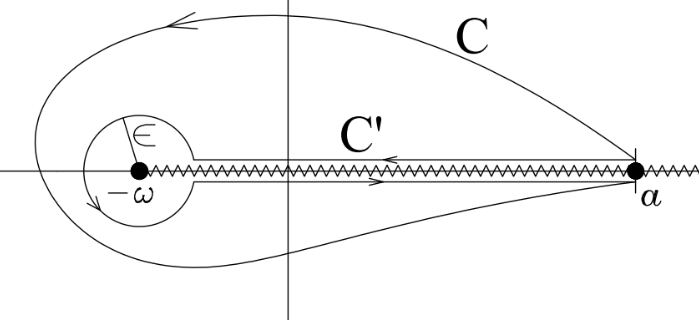
\includegraphics[width=.75\textwidth]{c32.PNG}
    \caption{The contour of integration with branch point at $-\omega$  and  branch  cut  runs  from $(-\omega,\infty)$.}
    \label{ch33}
\end{figure}

Lastly, to exactly evaluate the the generalized Stieltjes transform of the non-integral order
\begin{equation}\label{pf}
	S_{n+\alpha}^{a}[f(x)] = \int_{0}^{a}\frac{f(x)}{(\omega+x)^{n+\alpha}}\mathrm{d}x, 
\end{equation}
where $f(x)$ has an entire complex extension $f(z)$ and $\alpha$ is between $0$ and $1$. Again, we need to lift the integral to the complex plane. Doing so will induce a branch point at $z=-\omega$ and we choose that branch cut will run along the positive real axis. Now, consider a complex contour integral in the form of 
\begin{equation}
     \int_{C} \frac{f(z)}{(\omega + z)^{n+\alpha}} \mathrm{d}z ,
\end{equation}
where the contour $C$ is shown in the Figure \ref{ch33}. The contour will be deform to $C'$ and evaluating it will result to
\begin{eqnarray}\label{3.81}
\int_{C^\prime}\frac{f(z)}{(\omega+z)^{n+\alpha}}\mathrm{d}z&=&\int_a^{-\omega+\epsilon}\frac{f(x)}{(\omega+x)^{n+\alpha}}\mathrm{d}x + \int_{\epsilon}\frac{f(z)}{(\omega+z)^{n+\alpha}}\mathrm{d}z\nonumber\\\nonumber
&+&\int_{-\omega+\epsilon}^a\frac{f(x)}{(\omega+x)^{n+\alpha}e^{2\pi i(n+\alpha)}}\mathrm{d}x\\
&=&\int_a^{-\omega+\epsilon}\frac{f(x)}{(\omega+x)^{n+\alpha}}\mathrm{d}x+\int_{\epsilon}\frac{f(z)}{(\omega+z)^{n+\alpha}}\mathrm{d}z\\
 \quad & +&e^{-2\pi i\alpha}\int_{-\omega+\epsilon}^a\frac{f(x)}{(\omega+x)^{n+\alpha}}\mathrm{d}x\nonumber \\
&=&(e^{-2\pi i\alpha}-1)\int_{-\omega+\epsilon}^a\frac{f(x)}{(\omega+x)^{n+\alpha}}\mathrm{d}x+\int_{\epsilon}\frac{f(z)}{(\omega+z)^{n+\alpha}}\mathrm{d}z \nonumber
\end{eqnarray}
Combining the similar terms and using the parameterization $z = \epsilon\mathrm{e}^{i\theta}$, the resulting equation is
\begin{align}
\begin{split}
  \int_{C^\prime}\frac{f(z)}{(\omega+z)^{n+\alpha}}\mathrm{d}z &= (e^{-2\pi i\alpha}-1)\left [\int_{-\omega+\epsilon}^{0}\frac{f(x)}{(\omega+x)^{n+\alpha}}\mathrm{d}x+\int_{0}^{a}\frac{f(x)}{(\omega+x)^{n+\alpha}}\mathrm{d}x\right ]\\& \qquad +\int_{\epsilon}\frac{f(\epsilon \mathrm{e}^{i\theta} - \omega)}{(\epsilon \mathrm{e}^{i\theta})^{n+\alpha-1}}i\mathrm{d}\theta.
\end{split}
\end{align}
For the first term above, we will do a u-substitution technique. We will let $x = x' + \omega$, the first term will become
\begin{equation}
    \int_{-\omega+\epsilon}^{0}\frac{f(x)}{(\omega+x)^{n+\alpha}}\mathrm{d}x = \int_{\epsilon}^{\omega}\frac{f(x' - \omega)}{(x')^{n+\alpha}}\mathrm{d}x'.
\end{equation}
Dividing both sides by the factor $(e^{-2\pi i\alpha}-1)^{-1}$ and rearranging the terms such that we obtain the desired integral

\begin{align}
\begin{split}
 \int_0^a \frac{f(x)}{(\omega + x)^{n+\alpha}} \mathrm{d}x  & = \frac{1}{e^{-2\pi i\alpha}-1}\int_{C'}\frac{f(z)}{(\omega+z)^{n+\alpha}}\mathrm{d}z  
\\& \int_{\epsilon}^{\omega}\frac{f(x - \omega)}{(x)^{n+\alpha}}\mathrm{d}x -\frac{1}{e^{-2\pi i\alpha}-1} \int_{\epsilon}\frac{f(\epsilon \mathrm{e}^{i\theta} - \omega)}{(\epsilon \mathrm{e}^{i\theta})^{n+\alpha-1}}i\mathrm{d}\theta
\end{split}
\end{align}
To evaluate the the first term above, we will expand the binomial $(\omega+z)^{n+\alpha}$ with its binomial expansion at the origin given by
\begin{equation}
    \frac{1}{(\omega+z)^{n+\alpha}} = \sum_{k=0}^{\infty} {n+\alpha \choose k} \frac{\omega^{k}}{z^k+n+\alpha}
\end{equation}
Inserting this binomial expansion to the first term will give us
\begin{align}
\begin{split}
    \frac{1}{e^{-2\pi i\alpha}-1}\int_{C'}\frac{f(z)}{(\omega+z)^{n+\alpha}}\mathrm{d}z & =  \frac{1}{e^{-2\pi i\alpha}-1}\int_{C}\sum_{k=0}^{\infty} {n+\alpha \choose k} \omega^{k}\frac{f(z)}{(z)^{k+n+\alpha}}\mathrm{d}z \\& = \sum_{k=0}^{\infty} {n+\alpha \choose k} \omega^{k}  \frac{1}{e^{-2\pi i\alpha}-1}\int_{C} \frac{f(z)}{(z)^{k+n+\alpha}}\mathrm{d}z .
\end{split}
\end{align}
Again, similar to the previous section, the interchanging of order of the integration and summation is valid since the expansion and the contour is uniformly convergent for all $|z| > b$. It can also be shown formally by establishing a constant bound for the finite-part integral, by deforming the contour to a circle with radius a. Similar to the other section, it can established that the series is absolutely convergent for $\omega < a$. Now, invoking Theorem \ref{T3.2} the contour integral becomes
\begin{equation}
     \frac{1}{e^{-2\pi i\alpha}-1}\int_{C'}\frac{f(z)}{(\omega+z)^{n+\alpha}}\mathrm{d}z=\sum_{k=0}^{\infty} {n+\alpha \choose k} \omega^{k} \bbint{0}{a} \frac{f(z)}{(z)^{k+n+\alpha}}\mathrm{d}z 
\end{equation}
For the remaining terms which is dependent of $\epsilon$. It can be recognized that those terms is divergent at the origin. Lifting it to the contour integral and by the virtue of Theorem \ref{T3.2}, it will result to a finite-part integration
\begin{equation}
\bbint{0}{\omega}\frac{f(x-\omega)}{(x)^{n+\alpha}}\mathrm{d}x=\lim_{\epsilon\rightarrow0}\left[\int_{0}^{\omega-\epsilon}\frac{f(-x)}{(\omega-x)^{n+\alpha}}\mathrm{d}x-\frac{1}{e^{-2\pi i\alpha}-1} \int_{\epsilon}\frac{f(\epsilon \mathrm{e}^{i\theta} - \omega)}{(\epsilon \mathrm{e}^{i\theta})^{n+\alpha-1}}i\mathrm{d}\theta \right]
\end{equation}
Finally, we obtain a representation of the given integral presented in equation \eqref{pf} in terms of two finite part integral,
\begin{equation}\label{new}
\int_{0}^{a}\frac{f(x)}{(\omega+x)^{n+\alpha}}\mathrm{d}x=\sum_{k=0}^{\infty} {n+\alpha \choose k} \omega^{k} \bbint{0}{a} \frac{f(z)}{(z)^{k+n+\alpha}}\mathrm{d}z -\bbint{0}{\omega}\frac{f(x-\omega)}{x^{n+\alpha}}\mathrm{d}x.
\end{equation}
The finite-part integral arises from the singularity of the kernel of transformation will be called the progenic finite-part integrals. Evaluating further this progenic finite-part integrals, will result to
\begin{align}
\begin{split}
	\Delta_{\mathrm{sc}}^{(n+\alpha)} & (\omega) = \bbint{0}{\omega}\frac{f(x-\omega)}{x^{n+\alpha}}\mathrm{d}x
	\\& \quad= \sum_{j=0}^{\infty}\frac{f^{\left(j\right)}\left(-\omega\right) \,\omega^{j-n-\alpha+1}}{j!\,\left(j-n-\alpha+1\right)} .
\end{split}
\end{align}
The two equations above reproduce the theorem that can be found in \cite{tica2019finite}
\begin{theorem}\label{T3.5}
	Let $f(x)$ be locally integrable in the interval $[0,a]$ with an entire complex extension $f(z)$. Then
	\begin{equation}\label{new_rezult}
	\int_0^a\frac{f(x)}{(\omega+x)^{n+\alpha}}\mathrm{d}x=\sum_{j=0}^{\infty}{{-n-\alpha}\choose {j}}\, {\omega}^j \, \bbint{0}{a}\frac{f(x)}{x^{n+\alpha+j}}\mathrm{d}x + \Delta_{\mathrm{sc}}^{(n+\alpha)}(\omega),
	\end{equation}
	where $n=1,2,3...$ and $0<\alpha<1$, provided $\omega<a$, in which the singular contribution is the finite part integral
	\begin{align}
    \begin{split}\label{3.79}
	\Delta_{\mathrm{sc}}^{(n+\alpha)} & (\omega) =- \bbint{0}{\omega} \frac{f(-x)}{(\omega-x)^{n+\alpha}}\mathrm{d}x
	\\& \quad= \sum_{j=0}^{\infty}\frac{f^{\left(j\right)}\left(-\omega\right) \,\omega^{j-n-\alpha+1}}{j!\,\left(j-n-\alpha+1\right)} .
	\end{split}
    \end{align}
\end{theorem}

\section{Finite-part Integration in the Presence of Competing Singularities}

Now, we already see how the method is implemented to evaluate the Stieltjes transform. The theorems for the exact evaluation of the Stieltjes transform are only established for the functions with an entire complex extension. Recent development of the method is the application of finite-part integration to the Stieltjes transform of a function $f(x)$ with competing singularities when lifted to a complex plane.

According to \cite{doi:10.1063/5.0038274, lloydthetit}, the theorems presented from the previous section will still hold regardless of the nature of singularities that the complex extension of $f(x)$ possess, provided with some restriction. The first restriction comes from the desire to represent the contour integral as a finite-part integral. According to the conditions imposed by Theorem \ref{T3.1} and \ref{T3.2}, the contour should not enclose any singularities of $f(z)$. Also, it is specific that the contour $C$ should traverse the positive real axis of the complex plane as shown in Figure \ref{ch31}. Those conditions limit the possible choices of the complex extension of the function $f(z)$. For example, if $f(z)$ has a pole, then the pole must be located on the left-hand side of the complex plane since your contour is straddling along the positive real axis. Additionally, the branch cut of $f(z)$ should not overlap with the branch cut from the complex extension of the kernel of the transformation $(\omega + z)^{k+\nu}$. The second restriction comes from the method itself. Recall that to recover the missing terms from the term by term integration, the method requires the contour $C$ to enclose the singularity of the kernel located at $z=-\omega$. This requires the $\omega$ to be located not farther from the origin compared to the nearest singularity of $f(z)$. This implies that the radius of convergence of the infinite series in the right-hand side of the Theorems \ref{T3.3}, \ref{T3.4}, and $\ref{T3.5}$ is less than the distance of the nearest singularity of $f(z)$ with respect to the origin. Thus, the presence of singularities of $f(z)$ create a restriction on the radius of convergence of the infinite series of the finite-part integrals.

To appreciate it further, we will apply the method to the generalized Stietljes transform of $f(x) = (a+x)^{-\mu}$, which will have a singularity at $-a$. 

\subsection{Finite-part integration of the generalized Stieltjes transform of non-integral order}
In this case, we will evaluate the generalized Stieltjes transform of $f(x) = (a+x)^{-\mu}$ with non-integral order
\begin{equation}
    S_{m+\nu}[(a+x)^{-\mu}] = \int_{0}^{\infty} \frac{(a+x)^{-\mu}}{(\omega+x)^{m+\nu}} \mathrm{d}x, \quad 0<\nu<1.
\end{equation}
The divergence will be caused by the branch point singularity when the kernel expands at the origin. Moreover, when the integral is lifted to the complex plane, we will have a branch point singularity at $z=-\omega$ due to the kernel. We choose the branch cut to run along the positive real axis. Therefore, to solve the integral, we will consider the contour integral
\begin{equation}
    \int_{C} \frac{(a+z)^{-\mu}}{(\omega+z)^{m+\nu}} \mathrm{d}z.
\end{equation}

 \begin{figure}[t]
 	\centering
 	\includegraphics[width=0.75\textwidth]{c21.PNG}
 	 	\includegraphics[width=0.75\textwidth]{c12.PNG}
 	\caption{The deformation of the contour $\mathrm{C}$ to the contour $\mathrm{C}'$ to extract the Stieltjes integral. (Top) The point $z=-\omega$ is a branch point of the kernel transformation. (Bottom) The point $z=-\omega$ is a pole of the kernel of transformation. The point $z=-\tau$ is a branch point or a pole of the complex extension $f(z)$ of the function $f(x)$.}
 	\label{deformation}
 \end{figure}

The figure for the contour is obtained from \cite{doi:10.1063/5.0038274}.The top figure in Figure \ref{deformation} is the contour for the above expression. It is noticeable that the contour avoids the singularity of the function $f(z)$ or chosen to be far away from the origin, i.e., $a > \omega$. This translates to $\mu$ can be any positive number, or the nature of singularity of $f(z)$ would not matter. Deforming the contour to $C'$ as shown in the Figure \ref{deformation} and evaluate it, we will have
\begin{align}
\begin{split}
    \int_{C'} \frac{(a+z)^{-\mu}}{(\omega+z)^{m+\nu}}\,& \,\mathrm{d}z 
    = \left( e^{-2\pi i \nu}-1 \right) \int_{-\omega+\epsilon}^{\infty} \frac{ (a+x)^{-\mu}}{(b+x)^{m+\nu}} \, \mathrm{d}x 
    \\& + \int_{\epsilon} \frac{(a-\omega+\epsilon \mathrm{e}^{i\theta})^{-\mu}}{(\epsilon \mathrm{e}^{i\theta})^{m+\nu-1}}\, i \mathrm{d}\theta.
\end{split}
\end{align}
Recovering the Stietljes integral by rearranging the terms, and dividing both sides by $\left( e^{-2\pi i \nu}-1 \right)$, we will have
\begin{align}
\begin{split}
    \int_{0}^{\infty} \frac{ (a+x)^{-\mu}}{(b+x)^{m+\nu}} \, \mathrm{d}x  =  & \frac{1}{\left( e^{-2\pi i \nu}-1 \right)} \int_{C'} \frac{(a+z)^{-\mu}}{(\omega+z)^{m+\nu}} \,\mathrm{d}z \\& - \int_{-\omega+\epsilon}^{0} \frac{ (a+x)^{-\mu}}{(b+x)^{m+\nu}} \, \mathrm{d}x \\&  - \frac{1}{\left( e^{-2\pi i \nu}-1 \right)} \int_{\epsilon} \frac{(a-\omega+\epsilon \mathrm{e}^{i\theta})^{-\mu}}{(\epsilon \mathrm{e}^{i\theta})^{m+\nu-1}}\, i \mathrm{d}\theta.
\end{split}
\end{align}
Next, expanding the kernel of the contour integral at the origin and identify it as a finite-part integral using Theorem \ref{T3.1} will result to 
\begin{align}
\begin{split}
    \int_{0}^{\infty} \frac{ (a+x)^{-\mu}}{(\omega+x)^{m+\nu}} \, \mathrm{d}x  =  & \sum_{k=0}^{\infty} \binom{-m-\nu}{k} \omega^{k} \bbint{0}{\infty} \frac{(a+z)^{-\mu}}{z^{k+m+\nu}} \\& - \int_{-\omega+\epsilon}^{0} \frac{ (a+x)^{-\mu}}{(\omega+x)^{m+\nu}} \, \mathrm{d}x \\&  - \frac{1}{\left( e^{-2\pi i \nu}-1 \right)} \int_{\epsilon} \frac{(a-\omega+\epsilon \mathrm{e}^{i\theta})^{-\mu}}{(\epsilon \mathrm{e}^{i\theta})^{m+\nu-1}}\, i \mathrm{d}\theta.
\end{split}
\end{align}
For the remaining terms, we will perform a u-substitution $u = x+\omega$, and we will take the limit of $\epsilon \to 0$
\begin{align}
\begin{split}
    \int_{0}^{\infty} \frac{ (a+x)^{-\mu}}{(\omega+x)^{m+\nu}} \, \mathrm{d}x  =  & \sum_{k=0}^{\infty} \binom{-m-\nu}{k} \omega^{k} \bbint{0}{\infty} \frac{(a+z)^{-\mu}}{z^{k+m+\nu}} \\& - \lim_{\epsilon \to 0} \, \Bigg[ \int_{\epsilon}^{\omega} \frac{ (a-\omega+u)^{-\mu}}{u^{m+\nu}} \, \mathrm{d}u \\&  - \frac{1}{\left( e^{-2\pi i \nu}-1 \right)} \int_{\epsilon} \frac{(a-\omega+\epsilon \mathrm{e}^{i\theta})^{-\mu}}{(\epsilon \mathrm{e}^{i\theta})^{m+\nu-1}}\, i \mathrm{d}\theta \Bigg].
\end{split}
\end{align}
The remaining terms can be recognized that those terms are divergent at the origin. Lifting it to the contour integral and by virtue of Theorem \ref{T3.2}, it will result in a finite-part integration
\begin{align}
\begin{split}
\bbint{0}{\omega}\frac{f(x-\omega)}{x^{n+\alpha}}\,&\mathrm{d}x=\lim_{\epsilon\rightarrow0}\Bigg[\int_{0}^{\omega-\epsilon}\frac{f(-x)}{(\omega-x)^{n+\alpha}}\mathrm{d}x \\& \quad-\frac{1}{e^{-2\pi i\alpha}-1} \int_{\epsilon}\frac{f(\epsilon \mathrm{e}^{i\theta} - \omega)}{(\epsilon \mathrm{e}^{i\theta})^{n+\alpha-1}}i\mathrm{d}\theta \Bigg].
\end{split}
\end{align}
Finally, collecting all the results, we expressed the Stieltjes transform as a finite-part integral
\begin{align}
\begin{split}
    \int_{0}^{\infty} \frac{ (a+x)^{-\mu}}{(\omega+x)^{m+\nu}} \, \mathrm{d}x  =  & \sum_{k=0}^{\infty} \binom{-m-\nu}{k} \omega^{k} \bbint{0}{\infty} \frac{(a+z)^{-\mu}}{z^{k+m+\nu}} \\& - \bbint{0}{\omega} \frac{(a-\omega+x)^{-\mu}}{x^{m+\nu}}.
    \label{c2I1}
\end{split}
\end{align}
Obviously, the above equation can be obtained easily using theorem \ref{T3.5}. This confirmed the applicability of the theorem for the function with competing singularities.

To evaluate the first finite-part integral, we will consider it first as a usual integral with the bounds $\epsilon$ to $c$. We will determine the nature of each term (converging and diverging) at the limit $\epsilon \to 0$. to obtain the finite part value, we will drop the terms that will diverge and retain the converging terms. Lastly, we will evaluate the limit $c \to \infty$  to obtain the desired finite-part integral. 

Now, consider the finite-part integral as a usual integral with bounds $\epsilon$ and $c$. Then, we expand the $f(x)$ at the origin using the Taylor series expansion. The process will result to
\begin{equation}
    \int_{\epsilon}^{c}  \frac{(a+x)^{-\mu}}{x^{k+m+\nu}} \, \mathrm{d}x =  \int_{\epsilon}^{c} \sum_{l=0}^{\infty} \binom{-\mu}{l} \frac{1}{a^{k+\mu}} x^{l-k-m-\nu} \, \mathrm{d}x.
\end{equation}
The infinite series is absolutely convergence for $|x/a| < 1$. The convergence will permit the interchanging of the order of summation and integration. Performing a term by term integration, which will results to
\begin{equation}
    \int_{\epsilon}^{c}  \frac{(a+x)^{-\mu}}{x^{k+m+\nu}} \, \mathrm{d}x = \sum_{l=0}^{\infty} \binom{-\mu}{l} \frac{1}{a^{k+\mu}} \left. \frac{x^{l-k-m-\nu+1}}{l-k-m-\nu+1} \right|_{\epsilon}^{c}.
\end{equation}
Again, we can group the terms by taking the limits $\epsilon \to 0$. The terms from $0$ to $k+m-1$ that have a factor of $\epsilon$ will have diverging terms when $\epsilon \to 0$ since all the terms have a negative exponent. The rest of the terms will converge.  Doing so, we will have
\begin{align}
\begin{split} 
    C_\epsilon = & \sum_{l=0}^{\infty} \binom{-\mu}{l} \frac{1}{a^{k+\mu}} \frac{c^{l-k-m-\nu+1}}{l-k-m-\nu+1} \\& \quad -  \sum_{l=k+m}^{\infty} \binom{-\mu}{l} \frac{1}{a^{k+\mu}} \frac{c^{l-k-m-\nu+1}}{l-k-m-\nu+1},
\end{split}
\end{align}
\begin{equation}
    D_\epsilon =- \sum_{l=0}^{k+m-1} \binom{-\mu}{l} \frac{1}{a^{k+\mu}}  \frac{\epsilon^{l-k-m-\nu+1}}{l-k-m-\nu+1}. 
\end{equation}

Taking the limits $\epsilon \to 0$ and dropping the diverging terms will lead us to the value of finite-part integral 
\begin{align}
\begin{split} 
    \bbint{0}{c} \frac{(a+x)^{-\mu}}{x^{k+m+\nu}} \, \mathrm{d}x = \sum_{l=0}^{\infty} \binom{-\mu}{l} \frac{1}{a^{k+\mu}} \frac{c^{l-k-m-\nu+1}}{l-k-m-\nu+1},
\end{split}
\end{align}
the terms of the convergent group with $\epsilon$ factor will vanish since it will just approach 0. Now, it's time to take the limit $c \to \infty$. This will make the terms with negative powers vanished since a factor of $1/c \to 0$ as $c \to \infty$,
\begin{align}
\begin{split} 
    \bbint{0}{\infty} \frac{(a+x)^{-\mu}}{x^{k+m+\nu}} \, \mathrm{d}x = \lim_{c \to \infty} \sum_{l=k+m}^{\infty} \binom{-\mu}{l} \frac{1}{a^{k+\mu}} \frac{c^{l-k-m-\nu+1}}{l-k-m-\nu+1}.
\end{split}
\end{align}
The evaluate the limits, we will convert the infinite series to the form of hypergeometric function express in equation \eqref{GHF} and will consider its asymptotic expansion at the very large argument. In expressing the series as a hypergeometric function, we first need to ensure that the interval of the series start at zero, if not, shifting of the interval is needed to perform. Also, the pochammer symbol \cite[pg. 3, Eq. 1.1.1.2]{slater1966generalized}
\begin{equation}
    (a)_k = \frac{\Gamma(k+a)}{a}
\end{equation}
and the negative binomial theorem \cite{nbt}
\begin{equation}
    \binom{-\mu}{n} = (-1)^{n} \binom{n+\mu-1}{n} = (-1)^{n} \frac{\Gamma(n+\mu)}{\Gamma(n+1)\Gamma(\mu)},
\end{equation}
were needed in the algebraic manipulation of the series. Rewriting the series into hypergeometric function will result to
\begin{align}
\begin{split} 
    \bbint{0}{\infty} \frac{(a+x)^{-\mu}}{x^{k+m+\nu}} \, \mathrm{d}x & = \lim_{c \to \infty} \sum_{l=0}^{\infty} \binom{-\mu}{l+k+m} \frac{1}{a^{l+k+m+\mu}} \frac{c^{l-\nu+1}}{l-\nu+1}
    \\& 
    = \lim_{c \to \infty} \sum_{l=0}^{\infty} \frac{(-1)^{l+k+m} \Gamma(l+k+m+\mu)}{\Gamma(\mu)\Gamma(l+k+m+1)} \frac{1}{a^{l+k+m+\mu}} \frac{c^{l-\nu+1}}{l-\nu+1}
    \\& = \lim_{c \to \infty}\frac{(-1)^{k+m} c^{1-\nu}}{a^{k+m+\mu}} \frac{\Gamma(k+m+\mu) \Gamma(1-\nu)}{\Gamma(\mu)\Gamma(k+m+1)\Gamma(2-\nu)}
    \\& \qquad \times \sum_{l=0}^{\infty} \frac{(1)_{k} (k+m+\mu)_{l}(1-\nu)^{l}}{(m+1)_l(2-\nu)_l} \frac{(-c/a)^{l}}{l!}
    \\& = \lim_{c \to \infty}\frac{(-1)^{k+m} c^{1-\nu}}{a^{k+m+\mu}} \frac{\Gamma(k+m+\mu) \Gamma(1-\nu)}{\Gamma(\mu)\Gamma(k+m+1)\Gamma(2-\nu)}
    \\& \qquad \times \pFq{3}{2}{1, k+m+\mu,1-\nu}{k+m+1,2-\nu}{-\frac{c}{a}}.
\end{split}
\end{align}
The asymptotic expansion of ${}_3F_2$ at the very large argument \cite{wolfram} is written as
\begin{align}
\begin{split}
   \,& \pFq{3}{2}{a_1,a_2,a_3}{b_1.b_2}{-z} =  \\& \quad \quad  \frac{\Gamma(b_1) \Gamma(b_2)}{\Gamma(a_1) \Gamma(a_2) \Gamma(a_3)}  \Bigg( \frac{\Gamma(a_1) \Gamma(a_2-a_1) \Gamma(a_3-a_1)}{\Gamma(b_1-a_1) \Gamma(b_2-a_1) \Gamma(a_3)} (-z)^{-a_1} \left(  1+\mathcal{O} \left( \frac{1}{z} \right) \right) \\& \quad \quad \quad + \frac{\Gamma(a_2) \Gamma(a_1-a_2) \Gamma(a_3-a_2)}{\Gamma(b_1-a_2) \Gamma(b_2-a_2) \Gamma(a_3)} (-z)^{-a_2} \left(  1+\mathcal{O} \left( \frac{1}{z} \right) \right) \\& \quad \quad \quad \quad +  \frac{\Gamma(a_3) \Gamma(a_1-a_3) \Gamma(a_2-a_3)}{\Gamma(b_1-a_3) \Gamma(b_2-a_3) \Gamma(a_3)} (-z)^{-a_3} \left(  1+\mathcal{O} \left( \frac{1}{z} \right) \right) \Bigg) ,  |z| \to \infty.
\label{3F2simple} 
\end{split}
\end{align}
Since we will let $c \to \infty$, only the $z$ term with exponent $1-\nu$ will have a contribution
\begin{align}
\begin{split} 
    \bbint{0}{\infty} \frac{(a+x)^{-\mu}}{x^{k+m+\nu}} \, \mathrm{d}x &  =\frac{(-1)^{k+m}}{a^{k+m+\mu}} \frac{\Gamma(1-\nu)\Gamma(\nu)\Gamma(k+m+\mu+\nu-1)}{\Gamma(\mu) \Gamma(k+m+\nu)}.
\end{split}
\end{align}
Using the reflection relation of Gamma function \cite[p. 58-59]{hardy1940ramaniyan}
\begin{equation}
    \Gamma(z)\Gamma(1-z) = \frac{\pi}{\sin{\pi z}},
\end{equation}
the finite-part integral simplifies to
\begin{align}
\begin{split} 
    \bbint{0}{\infty} \frac{(a+x)^{-\mu}}{x^{k+m+\nu}} \, \mathrm{d}x &  = \frac{(-1)^{k+m}}{a^{k+m+\mu}} \frac{\pi}{\sin{\pi\nu}} \frac{\Gamma(k+m+\mu+\nu-1)}{\Gamma(\mu) \Gamma(k+m+\nu)}.
\end{split}
\end{align}
For the finite-part integral of the singular contribution, we will just do the same process. However, in this case, we only need to take the limit $\epsilon \to 0$ and change the lower limit to $\epsilon$. The change in variable for the upper limit is not needed since $\omega$ is only finite. Now, consider it as a usual integral and perform an expansion
\begin{equation}
    \int_{\epsilon}^{\omega} \frac{(a-\omega+x)^{-\mu}}{x^{m+\nu}} \, \mathrm{d}x = \int_{\epsilon}^{\omega} \sum_{k=0}^{\infty} \frac{1}{(a-\omega)^{k+\mu}} x^{k-m-\nu} \, \mathrm{d}x.
\end{equation}
It is certain that the summation is convergent for $|z| < |a-\omega|$. Therefore, the interchanging of the operators and term by term integration is allowed
\begin{equation}
    \int_{\epsilon}^{\omega} \frac{(a-\omega+x)^{-\mu}}{x^{m+\nu}} \, \mathrm{d}x = \sum_{k=0}^{\infty} \binom{-\mu}{k} \frac{1}{(a-\omega)^{k+\mu}} \left.  \frac{x^{k-m-\nu+1}}{k-m-\nu+1} \right|_{\epsilon}^{\omega}.
\end{equation}
Now, grouping the terms into converging and diverging group, we will have
\begin{align}
\begin{split} 
    C_\epsilon = & \sum_{k=0}^{\infty} \binom{-\mu}{k} \frac{1}{(a-\omega)^{k+\mu}} \frac{\omega^{k-m-\nu+1}}{k-m-\nu+1} \\& \quad -  \sum_{k=m}^{\infty} \binom{-\mu}{k} \frac{1}{(a-\omega)^{k+\mu}} \frac{\epsilon^{k-m-\nu+1}}{k-m-\nu+1},
\end{split}
\end{align}
\begin{equation}
    D_\epsilon = -\sum_{k=0}^{m-1} \binom{-\mu}{k} \frac{1}{(a-\omega)^{k+\mu}}  \frac{\epsilon^{k-m-\nu+1}}{k-m-\nu+1}. 
\end{equation}
To obtain the finite-part integral, we will now take the limit of $\epsilon \to 0$ and drop the diverging group, this will result to
\begin{align}
\begin{split} 
    \bbint{0}{\omega} \frac{(a-\omega+x)^{-\mu}}{x^{m+\nu}} \, \mathrm{d}x = & \sum_{k=0}^{\infty} \binom{-\mu}{k} \frac{1}{(a-\omega)^{k+\mu}} \frac{\omega^{k-m-\nu+1}}{k-m-\nu+1}.
\end{split}
\end{align}
The above series can be express in the form of hypergeometric function express in equation \eqref{GHF}, doing so will give us
\begin{align}
\begin{split} 
    \bbint{0}{\omega} \frac{(a-\omega+x)^{-\mu}}{x^{m+\nu}} \, \mathrm{d}x & =  \sum_{k=0}^{\infty} \frac{(-1)^{k}\Gamma(k+\mu)}{\Gamma(\mu)k!}  \frac{1}{(a-\omega)^{k+\mu}} \frac{\omega^{k-m-\nu+1}}{k-m-\nu+1}
    \\& = \frac{\omega^{1-m-\nu}}{\Gamma(\mu) (1-m-\nu)} \sum_{k=0}^{\infty} \frac{(\mu)_{k}(1-m-\nu)_k}{(2-m-\nu)_k k!} \left(\frac{\omega}{\omega-a}\right)^{k}
    \\& = \frac{\omega^{1-m-\nu}}{\Gamma(\mu) (1-m-\nu)} \pFq{2}{1}{\mu,1-m-\nu}{2-m-\nu}{\frac{\omega}{\omega-a}}.
\end{split}
\end{align}
Collecting all the result and substituting back to equation \eqref{c2I1}, we will have
\begin{align}
\begin{split}
    \int_{0}^{\infty} & \frac{ (a+x)^{-\mu}}{(\omega+x)^{m+\nu}} \, \mathrm{d}x \\& = \sum_{k=0}^{\infty} \binom{-m-\nu}{k} \omega^{k} \frac{(-1)^{k+m}}{a^{k+m+\mu}} \frac{\pi}{\sin{\pi\nu}} \frac{\Gamma(k+m+\mu+\nu-1)}{\Gamma(\mu) \Gamma(k+m+\nu)}  \\& \quad - \frac{\omega^{1-m-\nu}}{\Gamma(\mu) (1-m-\nu)} \pFq{2}{1}{\mu,1-m-\nu}{2-m-\nu}{\frac{\omega}{\omega-a}}.
\end{split}
\end{align}
We see that the infinite series of the first term is only absolutely convergent for $|\omega/a| < 1$. This is the effect of the singularities from the function $f(z)$. It limits the convergence of the result of the method. To access the region of $|\omega/a| > 1$, we will resort to the concept of analytic continuation. Therefore, we need to close the series to invoke the principle of an analytic function and extend the analyticity to a larger region. Closing the series means expressing the series to a known elementary/special function. Fortunately, the series can be close using the hypergeometric function with a form written in equation \eqref{GHF}. Doing so, we will have
\begin{align}
\begin{split}
    \int_{0}^{\infty} & \frac{(a+x)^{-\mu}}{(\omega+x)^{m+\nu}} \, \mathrm{d}x \\& = \frac{\pi}{\sin{\pi\nu}} \sum_{k=0}^{\infty} \frac{(-1)^{k}\Gamma(k+\mu+\nu)}{\Gamma(m+\nu)k!} \omega^{k} \frac{(-1)^{k+m}}{a^{k+m+\mu}}  \frac{\Gamma(k+m+\mu+\nu-1)}{\Gamma(\mu) \Gamma(k+m+\nu)}  \\& \quad - \frac{\omega^{1-m-\nu}}{\Gamma(\mu) (1-m-\nu)} \pFq{2}{1}{\mu,1-m-\nu}{2-m-\nu}{\frac{\omega}{\omega-a}}.
    \\&= \frac{\pi}{\sin{\pi\nu}} \frac{(-1)^{m} \Gamma(m+\mu+\nu-1)}{\Gamma(\mu) \Gamma(m+\nu)a^{m+\mu}} \sum_{k=0}^{\infty}  \frac{(m+\mu+\nu-1)_{k} (\omega/a)^{k}}{k!}  \\& \quad - \frac{\omega^{1-m-\nu}}{\Gamma(\mu) (1-m-\nu)} \pFq{2}{1}{\mu,1-m-\nu}{2-m-\nu}{\frac{\omega}{\omega-a}}.
\end{split}
\end{align}
Finally, we successfully evaluate the Stieltjes transform of $(a-x)^{-\mu}$ of non-integral order
\begin{align}
\begin{split}
    \int_{0}^{\infty} & \frac{(a+x)^{-\mu}}{(\omega+x)^{m+\nu}} \, \mathrm{d}x \\& = \frac{\pi}{\sin{\pi\nu}} \frac{(-1)^{m} \Gamma(m+\mu+\nu-1)}{\Gamma(\mu) \Gamma(m+\nu)a^{m+\mu}} \pFq{1}{0}{m+\mu+\nu-1}{-}{\frac{\omega}{a}}  \\& \quad - \frac{\omega^{1-m-\nu}}{\Gamma(\mu) (1-m-\nu)} \pFq{2}{1}{\mu,1-m-\nu}{2-m-\nu}{\frac{\omega}{\omega-a}}.
\end{split}
\end{align}
The above result was already presented in \cite{Villanueva_Galapon_2019}.

We can see here the necessity to close the infinite series to access the region $a < \omega$ that restricts by the singularity of the complex extension of $f(x)$.

%%%%%%%%%%%%%%%%%%%%%%%%%%%%%%%%%%%%%%%%%%%%%%%%%%%%%%%%%%%%%%%%%%%%

\subsection{Finite-part integration of the generalized Stieltjes transform of integral order}
Lastly, we will consider the integral order of the generalized Stieltjes transform of $f(x) = (a+x)^{-\mu}$
\begin{equation}
    S_{m}[(a+x)^{-\mu}] = \int_{0}^{\infty} \frac{(a+x)^{-\mu}}{(\omega+x)^{m}} \mathrm{d}x.
\end{equation}
If we naively expand the kernel at the origin, the divergence is caused by the pole singularity. Also, the singularity due to the kernel is a pole singularity. With that, we need to induce a branch cut that runs along the positive real axis, and it can be induced by the complex extension of $\log x$. From that, we will consider the contour integral 
\begin{equation}
    \int_C \frac{(a+z)^{-\mu}}{(\omega +z )^{m}} \log{z} \, \mathrm{d}z,
\end{equation}
where the contour is the bottom figure of Figure \ref{deformation}. From the chosen contour, where we avoid the singularity of $f(z)$, we see that we pick $a$ to be very far away from the origin or at least $|a| > |\omega|$. In this condition, the nature of singularity of $f(z)$ would not matter. 

Similar to previous example, we will evaluate the deformed contour and extract the Stieltjes transform we want to evaluate
\begin{align}
\begin{split}
    \int_0^\infty \frac{(a+x)^{-\mu}}{(\omega+x)^m} \, \mathrm{d}x & = \frac{1}{2 \pi i} \int_C \frac{(a+z)^{-\mu}}{(\omega + z)^{m}} \, \left[ \log(z) -\pi i \right]\mathrm{d}z \\& \qquad - \mathrm{Res} \left[ \frac{ (a+z)^{-\mu}}{(\omega+z)^{m}}\, (\log(z) - \pi i)\right]_{z=-\omega}.
\end{split}
\end{align}
Expanding the kernel in the contour integral and we can express it as a finite-part integral by the virtue of Theorem \ref{T3.1}., we will have
\begin{align}
\begin{split}
    \int_0^\infty \frac{(a+x)^{-\mu}}{(\omega+x)^m} \, \mathrm{d}x & = \sum_{k=0}^{\infty} {-m \choose k} b^{k}   \bbint{0}{\infty} \frac{(a+x)^{-\mu}}{x^{k+m}} \mathrm{d}x \\& \qquad - \mathrm{Res} \left[ \frac{ (a+z)^{-\mu}}{(\omega+z)^{m}}\, (\log(z) - \pi i)\right]_{z=-\omega}.
\end{split}
\end{align}


Also, using equation \eqref{Res} we can easily evaluate the residue
\begin{align}
\begin{split} \label{SC}
    \mathrm{Res} \left[ \frac{(a+z)^{-\mu}}{(\omega+z)^{m}}\, \log(-z)\right]_{z=-\omega} = \,& \frac{(2-\mu-m)_{m-1}}{\Gamma(m) \, (a-\omega)^{\mu+m-1}} \, \log (\omega) \\& \hspace{-40mm} + \sum_{k=1}^{m-1} {m-1 \choose k} \frac{(-1)^k \Gamma(k)}{\omega^k} \frac{(2-\mu-m+k)_{m-1-k}}{(a-\omega)^{\mu+m-k-1}}.
\end{split}
\end{align}

Now, we will evaluate the finite-part integral. Again, we change its limit and treat it as a usual integral. Moreover, we expand the $(a+x)^{-\mu}$ with the convergence $|x/a|<1$ and interchange the order of summation and integration
\begin{equation}
    \int_{\epsilon}^{c} \frac{(a+x)^{-\mu}}{x^{k+m}} \, \mathrm{d}x = \sum_{l=0}^{\infty} \binom{-\mu}{l} \frac{1}{a^{l+\mu}} \int_{\epsilon}^{c} x^{l-k-m} \, \mathrm{d}x.
\end{equation}
Similar to the previous example, the interchanging of operators is allowed by the convergence of the series. Next, we will group the terms depending if they will converge or diverge when the limit $\epsilon \to 0$ is taken. For sure, negative integers of $\epsilon$ will diverge, which can be found in the interval $0 \leq l \leq k+m-2$. The term $l = k+m-1$ will also converge as $\epsilon \to 0$ since this is evaluated as a logarithm. Therefore, the groups are
\begin{align}
\begin{split} 
    C_\epsilon = & \sum_{l=k-m-2}^{\infty} \binom{-\mu}{l} \frac{1}{a^{k+\mu}} \frac{c^{l-k-m+1}}{l-k-m+1} + \binom{-\mu}{k+m-1} \frac{\ln{c}}{a^{k+m-1+\mu}} \\& \quad +\sum_{l=k-m}^{\infty} \binom{-\mu}{l} \frac{1}{a^{k+\mu}} \frac{c^{l-k-m+1}}{l-k-m+1} \\& \quad  -  \sum_{l=k+m}^{\infty} \binom{-\mu}{l} \frac{1}{a^{l+\mu}} \frac{\epsilon^{l-k-m-\nu+1}}{l-k-m-\nu+1},
\end{split}
\end{align}
\begin{align}
\begin{split} 
    D_\epsilon & = - \binom{-\mu}{k+m-1} \frac{\ln{\epsilon}}{a^{k+m-1+\mu}} \\& \qquad - \sum_{l=0}^{k+m-2} \binom{-\mu}{l} \frac{1}{a^{l+\mu}}  \frac{\epsilon^{l-k-m+1}}{l-k-m+1}. 
\end{split}
\end{align}
To obtain the finite-part integral, we will take the limit $\epsilon \to 0$ and disregard the diverging part. The $\epsilon$ with positive exponent will just approach zero
\begin{align}
\begin{split} 
    \bbint{0}{c} & \frac{(a+x)^{-\mu}}{x^{k+m}} \, \mathrm{d}x =  \sum_{l=0}^{k-m-2} \binom{-\mu}{l} \frac{1}{a^{l+\mu}} \frac{c^{l-k-m+1}}{l-k-m+1} \\& \quad + \binom{-\mu}{k+m-1} \frac{\ln{c}}{a^{k+m-1+\mu}}  +\sum_{l=k-m}^{\infty} \binom{-\mu}{l} \frac{1}{a^{l+\mu}} \frac{c^{l-k-m+1}}{l-k-m+1}
\end{split}
\end{align}
Now we take the limit $c \to \infty$, the terms with negative exponents will just vanish when evaluated. 
\begin{align}
\begin{split} \label{F1}
    \bbint{0}{\infty} \frac{(a+x)^{-\mu}}{x^{k+m}} \, \mathrm{d}x =  \lim_{c \to \infty} & \Bigg[ \sum_{l=k+m}^{\infty} \binom{-\mu}{l} \frac{1}{a^{l+\mu}} \frac{c^{l-k-m+1}}{l-k-m+1} \\& \qquad + \binom{-\mu}{k+m-1} \frac{\ln{c}}{a^{k+m-1+\mu}} \Bigg].
\end{split}
\end{align}
To evaluate the limits, we will obtain the closed form expression of the series, which is a hypergeometric function found in equation \eqref{GHF} 
\begin{align}
\begin{split} 
    \sum_{l=k+m}^{\infty} & \binom{-\mu}{l}  \frac{1}{a^{l+\mu}} \frac{c^{l-k-m+1}}{l-k-m+1} 
    \\&  = \sum_{l=0}^{\infty} \binom{-\mu}{l+k+m} \frac{1}{a^{l+k+m+\mu}} \frac{c^{l+1}}{l+1} 
    \\&  = \frac{c}{a^{k+m+\mu}} \sum_{l=0}^{\infty} \frac{(-1)^{l+k+m}\Gamma(l+k+m+\mu)}{\Gamma(\mu)\Gamma(l+k+m+1)(l+1)} \left(\frac{c}{a}\right)^{l} 
    \\& = \frac{(-1)^{k+m}c^{-1}}{a^{k+m+\mu}\Gamma(\mu)} \frac{\Gamma(k+m+\mu)}{\Gamma(k+m+1)} \sum_{l=0}^{\infty}  \frac{ (1)_{l} (1)_{l} (k+m+\mu)_l }{(k+m+1)_l (2)_l l!} \left(\frac{-c}{a}\right)^{l} 
    \\& = \frac{(-1)^{k+m}c^{-1}}{a^{k+m+\mu}\Gamma(\mu)} \frac{\Gamma(k+m+\mu)}{\Gamma(k+m+1)} \pFq{3}{2}{1,1,k+m+\mu}{2, k+m+1}{\frac{-c}{a}},
\end{split}
\end{align}
and use its asymptotic expansion at very large argument. The asymptotic expansion of ${}_3 F_2$ with a double pole for a large argument is given by
\begin{align}
\begin{split} \label{3F2doublepole}
    \,& \pFq{3}{2}{a_1,a_1,a_2}{b_1,b_2}{-z}   = \frac{\Gamma(b_1) \Gamma(b_2) \Gamma^2(a_1-a_3)} {\Gamma^2(a_1) \Gamma(b_1-a_3) \Gamma(b_2-a_3)} (-z)^{-a_3} \left( 1+\mathcal{O} \left( \frac{1}{z} \right) \right) \\& \quad + \frac{\Gamma(b_1) \Gamma(b_2) \Gamma(a_3-a_1)}{\Gamma(a_1) \Gamma(a_3) \Gamma(b_1-a_1) \Gamma(b_2-a_1)}  (\log(-z)+\psi(a_3-a_1)-\psi(b_1-a_1) \\& \quad \quad -\psi(b_2-a_1)-\psi(a_1)-2\gamma) (-z)^{-a_1} \left( 1+\mathcal{O} \left( \frac{1}{z} \right) \right), |z| \to \infty
\end{split} 
\end{align}
where $\psi(x)$ is a digamma function and $\psi(1) = -\gamma$ is the Euler-Masheroni constant \cite{wolfram1}. The first term will vanished since your $c$ will have a negative exponent, thus will approach to zero. Your second term will only contribute as $c \to \infty$ since the $c$ will cancel out
\begin{align}
\begin{split} 
    \sum_{l=k+m}^{\infty} & \binom{-\mu}{l}  \frac{1}{a^{l+\mu}} \frac{c^{l-k-m+1}}{l-k-m+1} 
    \\& = \frac{(-1)^{k+m}c^{-1}}{a^{k+m+\mu-1}\Gamma(\mu)}  \frac{\Gamma(1-k-m-\mu)}{\Gamma(k+m)} 
    \\& \qquad \times (\ln{(c/a)} + \psi(k+m+\mu-1) - \psi(k+m)).
\end{split}
\end{align}
Also, bringing  back the above equation to equation \eqref{F1}, the $\ln{c}$ will cancel out. The resulting finite-part integral is 
\begin{align}
\begin{split} 
    \bbint{0}{\infty} \frac{(a+x)^{-\mu}}{x^{k+m}} \,& \mathrm{d}x = \frac{1}{a^{k+m+\mu-1}}{-\mu \choose k+m-1} \\& \times \left(\ln(a) + \psi(k+m) - \psi(k+m+\mu-1) \right).
\label{FPIfinal}
\end{split}
\end{align}
Combining all the results, we will obtain 
\begin{align}
\begin{split} \label{22}
    &  \int_0^\infty \frac{(a+x)^{-\mu}}{(\omega+x)^m} \, \mathrm{d}x  = \sum_{k=0}^{\infty} {-\rho \choose k} \left( \frac{b}{a} \right)^{k} \frac{1}{a^{\rho+\mu-1}}{-\mu \choose k+\rho-1} \\&  \hspace{20 mm}\times \left(\log(a) + \psi(k+\rho) - \psi(k+\rho+\mu-1) \right) \\& - \left[ \frac{(2-\mu-\rho)_{\rho-1}}{\Gamma(\rho) \, (a-b)^{\mu+\rho-1}} \, \ln (b) - \sum_{k=1}^{\rho-1} {\rho-1 \choose k} \frac{ \Gamma(k)}{b^k} \frac{(2-\mu-\rho+k)_{\rho-1-k}}{(a-b)^{\mu+\rho-k-1}} \right].
\end{split}
\end{align}
Using binomial expansion on $(a-b)^{\mu+\rho-1}$ the coefficient of $\ln{b}$, we can readily see that the it is equal to the coefficient of $\ln{a}$. Therefore, we can combine the two terms leading the expression
\begin{align}
\begin{split}
    &  \int_0^\infty \frac{(a+x)^{-\mu}}{(\omega+x)^m} \, \mathrm{d}x  = \sum_{k=0}^{\infty} {-\rho \choose k} \left( \frac{b}{a} \right)^{k} \frac{1}{a^{\rho+\mu-1}}{-\mu \choose k+\rho-1} \\&  \hspace{20 mm}\times \left(\log(a)+ \psi(k+\rho) - \psi(k+\rho+\mu-1) \right) \\& - \left[ \frac{(2-\mu-\rho)_{\rho-1}}{\Gamma(\rho) \, (a-b)^{\mu+\rho-1}} \, \ln {\frac{b}{a}} - \sum_{k=1}^{\rho-1} {\rho-1 \choose k} \frac{ \Gamma(k)}{b^k} \frac{(2-\mu-\rho+k)_{\rho-1-k}}{(a-b)^{\mu+\rho-k-1}} \right].
\end{split}
\end{align}
The infinite series from the evaluated finite-part integration is again only convergent for $|b/a| < 1$. It is necessary to obtain a close form of this summation to access the region outside the convergence. This summation of the digamma function is expected to arise naturally in calculating the finite-part integral for the pole singularity case since we are most of the time using the double pole case of the asymptotic expansion of ${}_3F_2$. Therefore, it is necessary to study this hypergeometric-type series containing a digamma function as a factor.